\documentclass[
  final,
  babelLanguage=portuguese,
  %desktopVersion,
  %showtrims,
  %overleaf,
]{anecdote}

\graphicspath{{./assets/photos/300dpi/}}

% Page size: 6x9 inch
% Body text: 10.5 / 15 pt

\usepackage{local}

%% Details of the book
%% ===================

\title{Quatro Nobres Verdades}
\subtitle{}
\author{Ajahn Sumedho}
\publisher{Publicações Sumedhārāma}
\date{2018-07-23}
\editionInfo{\emph{Segunda Edição}, impresso na Malásia, 2019}
\ISBN{000-000-0000-00-0}% TODO update ISBN

% === Metadata ===

\hypersetup{
  pdftitle={\thetitle},
  pdfauthor={\theauthor},
  pdfcopyright={Copyright (C) 2019, \thePublisher},
  pdfsubject={},% TODO subject
  pdfkeywords={},% TODO keywords
  pdflicenseurl={https://creativecommons.org/licenses/by-nc-nd/4.0/},
  pdfcontacturl={},
  pdflang={pt},
}

% FIXME macro missing from LuaTeX 2018
%\pdfinfo{%
%  /Title (\thetitle)%
%  /Author (\theauthor)
%  /Subject (subject)% TODO subject
%  /Keywords (keywords)% TODO keywords
%  /GTS_PDFXVersion (PDF/X-1:2001)%
%  /GTS_PDFXConformance (PDF/X-1a:2001)%
%}

%% === Load further packages ===

%% === Hyphenation exceptions and corrections ===

\hyphenation{London}

\begin{document}

\frontmatter

\ifdesktopversion
\desktopCover{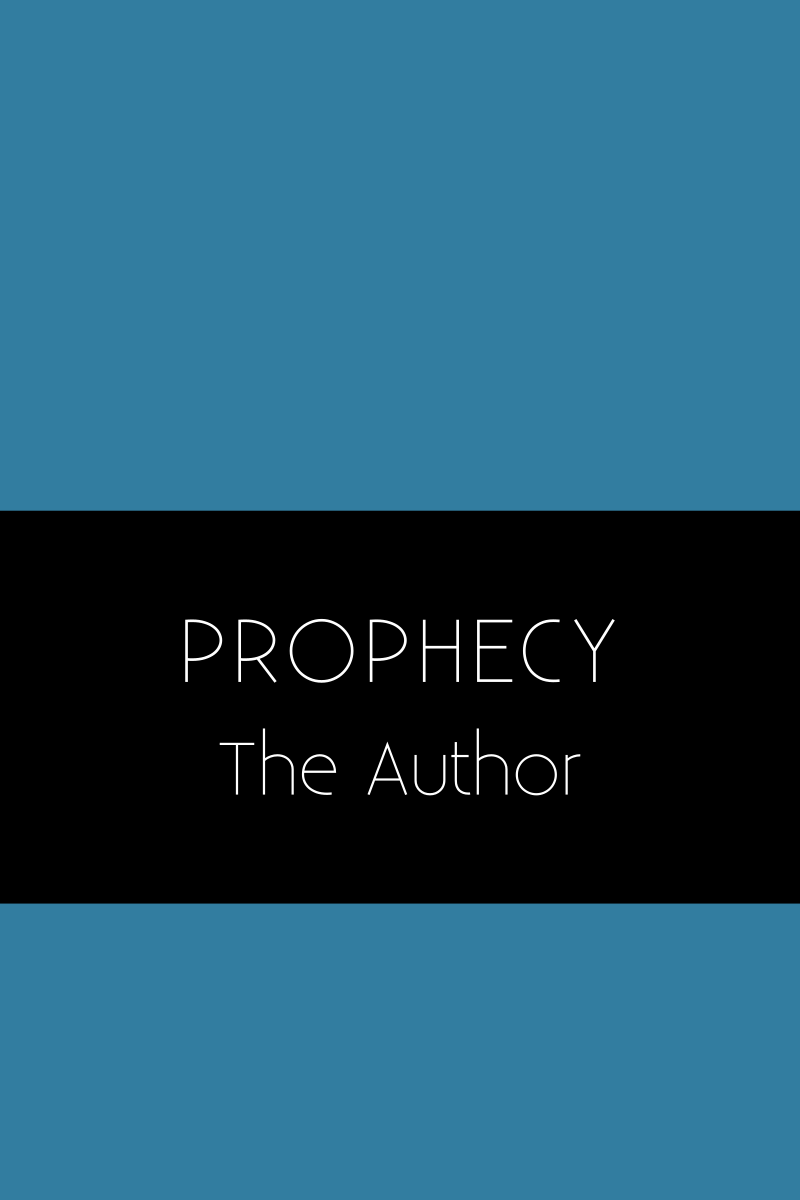
\includegraphics[height=\paperheight]{./desktop-cover.png}}
\fi

\cleartorecto
\thispagestyle{empty}
\vspace*{5em}

{\centering

\settowidth{\titleLength}{%
  {\Large\crimsonRomanFont\scshape\thetitle}%
}

{\Large\crimsonRomanFont\scshape\thetitle}\\[0.3\baselineskip]
\setlength{\xheight}{\heightof{X}}
\raisebox{0.5\xheight}{\color[gray]{0.4}\rule{\titleLength}{0.25pt}}\\[0.3\baselineskip]
{\itshape
\thesubtitle}

\vfill

\theauthor

\vspace*{5em}

}



\cleartoverso
\thispagestyle{empty}

{\copyrightsize
\centering
\setlength{\parindent}{0pt}%
\setlength{\parskip}{0.8\baselineskip}%

\thetitle\ -- \thesubtitle\\
by \theauthor

Published by \thePublisher

ISBN \theISBN

Copyright \copyright\ \thePublisher\ 2017

Cover Photograph: The Person

\vfill

{\footnotesize

This work is licensed under a Creative Commons\\
Attribution-NonCommercial-NoDerivatives 4.0 International~License.

Produced with the \LaTeX\ typesetting system, set in Gentium and Crimson Roman.

\theEditionInfo

}}


\cleartorecto
\thispagestyle{empty}

\mbox{}\vfill

\begin{verse}
\centering
Dedicação

\bigskip

Gostaríamos de deixar o nosso agradecimento a todos aqueles que
contribuíram para a preparação deste livro, e em particular ao grupo
Kataññuta da Malásia, Singapura e Austrália por tornar possível esta~publicação.

\sectionBreak

Dedicado também com gratidão aos meus pais. E à
saudosa memória de minha avó Elisa, que ela possa realizar a
paz do Nibbāna.

Kāñcano Bhikkhu

\end{verse}

\vfill\mbox{}


\cleartorecto
\tableofcontents*

\newpage\mbox{}
\thispagestyle{empty}
\newpage\mbox{}
\thispagestyle{empty}

\makeatletter
\AddToShipoutPictureFG*{%
  \put(\LenToUnit{-3mm},\LenToUnit{-3mm}){%
  %
  \begin{tikzpicture}
    \node (bg) [
      minimum width = \BOOK@paperWidth + 6mm,
      minimum height = \BOOK@paperHeight + 6mm,
    ] {};
    %
    \node (title) [
      minimum width=\BOOK@paperWidth + 6mm,
      below right=18mm and 0pt of bg.north west,
    ] {%
      \begin{minipage}{\BOOK@paperWidth}%
        \centering
        {%
          \chapterTitleFont\chapterTitleSize\color{chaptertitle}%
          Uma Mão Cheia de Folhas%
        }%
      \end{minipage}%
    };%
    %
    \node (quote) [
      minimum width=\BOOK@paperWidth + 6mm,
      below right=8mm and 0pt of bg.mid,
      anchor=mid,
    ] {%
      \begin{minipage}{90mm}%
        \setlength{\parindent}{0pt}%
        \setlength{\parskip}{5pt}%
\vspace*{0.5\onelineskip}%
\fontsize{10}{13}\selectfont%
\color{chapternote}%

A certa altura, estando O Iluminado a viver em Kosambi numa floresta de
Siṃsapās, pegou numa mão cheia de folhas e perguntou aos monges,

«Monges, o que pensam disto? O que é mais numeroso, as poucas folhas
que tenho na mão ou aquelas nas árvores desta floresta?».

«As folhas que O Iluminado tem na mão são poucas, Senhor; as da floresta são
bastante mais numerosas».

«Assim também, monges, as coisas que eu aprendi por conhecimento directo são
bastante numerosas; as coisas que eu vos ensinei são poucas.

E porque é que eu não ensinei todas? Porque elas não trazem qualquer benefício,
nem desenvolvimento na Vida Santa, porque não conduzem ao fim da ilusão, ao
despojamento, à cessação, ao acalmar, ao conhecimento directo, à iluminação, à
libertação. Por essa razão não as ensinei.

E o que é que eu vos ensinei? Existe o sofrimento; existe a origem do
sofrimento; existe o cessar do sofrimento; existe o caminho que conduz à
cessação do sofrimento. Isto foi o que vos ensinei.

E porque é que eu ensinei isto? Porque traz benefício e desenvolvimento na Vida
Santa, porque conduz ao fim da ilusão, ao despojamento, à cessação, ao acalmar,
ao conhecimento directo, à iluminação, à libertação.

Assim sendo monges, que esta seja a vossa tarefa: Existe o sofrimento; existe a
origem do sofrimento; existe o cessar do sofrimento; existe o caminho que leva à
cessação do sofrimento».

\quoteRef{Saṃyutta Nikāya 56.31}

\vspace*{0.5\onelineskip}%

      \end{minipage}%
    };%
    %
    \node (topbox) [
      minimum width=\BOOK@paperWidth + 6mm,
      minimum height=10pt,
      above=1mm of quote.north,
      anchor=south,
    ] {};
    %
    \draw [line width=2pt, draw=black!40]
      (topbox.north west) -- (topbox.north east);
    %
    \draw [line width=1pt, draw=black!40, dash pattern=on 1pt off 5pt]
      (topbox.south west) -- (topbox.south east);
    %
    \node (bottombox) [
      minimum width=\BOOK@paperWidth + 6mm,
      minimum height=10pt,
      below=1mm of quote.south,
      anchor=north,
    ] {};
    %
    \draw [line width=1pt, draw=black!40, dash pattern=on 1pt off 5pt]
      (bottombox.north west) -- (bottombox.north east);
    %
    \draw [line width=2pt, draw=black!40]
      (bottombox.south west) -- (bottombox.south east);
    %
  \end{tikzpicture}%
}}%
\makeatother



\chapter{Nota do Tradutor}

Gostaria, em primeiro lugar, de apresentar o meu especial
e respeitoso agradecimento ao Venerável Ajahn Sumedho, pelo
encorajamento e pela disponibilidade que demonstrou no
decorrer deste trabalho de tradução. Como português estou
grato também, pelo entusiasmo e alegria que manifesta ao
aceitar os convites vindos de Portugal para aí divulgar o
Dhamma. Em “Anjali”.
O custo desta edição foi mais uma vez patrocinado na sua
íntegra por Gene Lushtak. “Sādhu Anumodanā”, prezado
amigo obrigado, pela tua grande generosidade, empenho e
constante entusiasmo na divulgação do Dhamma.
Um especial agradecimento ao meu bom amigo
Samanera Appāmado, companheiro neste caminho espiritual,
que durante vários meses me apoiou e encorajou na realização deste projecto, sempre com enorme entusiasmo, energia e
bom humor.
Não posso de modo algum deixar também de mencionar a
incansável colaboração das amigas e compatriotas, Anagarikā
Ana Sofia e Sofia Gallis, membros da presente comunidade em
Amarāvatī, pelo empenho e valiosa contribuição para a concretização desta tradução. Sem dúvida este esforço conjunto
engrandeceu este projecto.

Que a Luz do Dhamma e os meritórios frutos das vossas
acções vos iluminem e protejam no caminho para a plenitude
e libertação de todo o sofrimento.

Kāñcano Bhikkhu
Mosteiro Amarāvatī
Outubro 2007

\chapter{Prefácio}

\thispagestyle{bottomcenter}

Este livro foi compilado e editado a partir de palestras proferidas pelo
Venerável Ajahn Sumedho sobre o ensinamento essencial do Buddha - que a
infelicidade humana pode ser transcendida através do caminho espiritual.

A primeira exposição das Quatro Nobres Verdades foi apresentada pelo Buddha, em
528 a.C., no Parque dos Cervos em Sarnāth, perto de Varanāsi, através do
discurso \emph{Sutta Dhammacakkappavattana} – que literalmente
significa “o discurso que coloca em movimento o veículo do ensinamento”.
Excertos deste \emph{sutta} são citados no início de cada capítulo, descrevendo
as Quatro Nobres Verdades. Cada referência corresponde à secção dos livros das
escrituras (Pāli Cânon), onde este discurso pode ser encontrado. No entanto, nas
escrituras, o tema das Quatro Nobres Verdades repete"-se algumas vezes, como por
exemplo na citação que aparece no início da Introdução.

Em muitas das suas palestras Ajahn Sumedho usa a expressão budista de “not"-self”
(\emph{anattā}) “não eu”. Ajahn Sumedho ensina que a raiz da ignorância é a
ilusão da existência de um eu. Desta forma, não está a falar de aniquilação ou
da rejeição das qualidades pessoais, mas sim a indicar como o sofrimento
(\emph{dukkha}) surge quando querermos manter esta identificação com o corpo e
com a mente, sendo esta identificação errada aquilo a que a maioria das
pessoas chama de “eu”.

Outro termo usado muitas vezes por Ajahn Sumedho nas suas palestras é
“deathless”, que surge neste livro com alguma frequência. Por não existir em
português uma única palavra que ilustre claramente o seu significado, foi
traduzido de diferentes formas, usando"-se os termos que melhor se adequavam ao
contexto de cada situação. Podemos ainda acrescentar que a palavra se refere,
não ao sentido de imortalidade mas sim àquilo que está para além do ciclo de
vida e de morte, não em termos metafísicos mas sim no sentido de impermanência -
“Tudo o que surge está sujeito a cessar” – não se tratando portanto da
derradeira realidade. Nas escrituras existe uma passagem que pode ajudar a
clarificar um pouco mais a palavra “deathless”:

\begin{quote}
  «Existe, bhikkhus, um não nascido, não formado, incriado, o originado. 
  Se não existisse este não nascido, não formado, incriado, não
  originado, não existiria o nascido, o formado, o criado e o originado. Porém,
  precisamente porque existe um não nascido, não formado, incriado e não
  originado, é possível a libertação do nascido, formado, criado e originado».

  \quoteRef{Nibbāna Sutta, Ud 8.3}
\end{quote}

Luang Por Sumedho oferece"-nos a seguinte reflexão sobre esta profunda
declaração: «Podemos ver que não somos vítimas prisioneiras da condição do
nascimento, sem qualquer esperança de escaparmos ao sofrimento da mudança, dos
nossos hábitos e desejos. Existe, assim, uma saída: realizar a existência do não
nascido, não formado, incriado, não originado. Reconhecer, isso é \emph{sati
  sampajaññā}, \emph{sati paññā} ou consciência.

É perceber a diferença entre
estar e não estar apegado à forma, ao que é criado. Nibbāna é a realidade do
não"-apego aos fenómenos condicionantes; não se trata de destruir o
\emph{saṃsāra}, de aniquilar todos as condições por estas serem tão limitadoras
e só conduzirem ao sofrimento, mas sim de reconhecer e discernir essa realidade».

Concluindo, estas Quatro Nobres Verdades são como que um exercício de
discernimento; ajudam a não tomar posições rígidas a favor ou contra o que quer
que seja, mas sim a reconhecer o Não Nascido e Não Criado como verdadeiro, e não
como uma fantasia ou um ideal. Desta forma, esta realidade é reconhecida e
cultivada na nossa vida quotidiana.

Caro leitor, o desejo é que, ao explorar as seguintes páginas, os corações de
todos aqueles que tiveram a oportunidade de encontrar a sabedoria dos
ensinamentos aqui contidos, se sintam inspirados a despertar, e rapidamente
realizem o fim de todo o sofrimento.

\bigskip

{\raggedleft
  Kāñcano Bhikkhu\\
  Mosteiro Amarāvatī\\
  Outubro 2007
\par}



\chapter{Introdução}

\begin{quote}
  «A razão porque, quer Eu, quer vocês, viajámos e deambulámos durante muito
  tempo neste longo ciclo, deve-se a não termos descoberto nem penetrado quatro
  verdades. Quais são?

  São: A Nobre Verdade do Sofrimento, A Nobre Verdade da Origem do Sofrimento, A
  Nobre Verdade do Cessar do Sofrimento e A Nobre Verdade do Caminho que conduz
  à Cessação do Sofrimento».

  \quoteRef{Dīgha Nikāya 16}
\end{quote}

O \emph{Sutta Dhammacakkappavattana}, o ensinamento do Buddha acerca das Quatro
Nobre Verdades, tem sido a principal referência que tenho usado na minha prática
ao longo dos anos. É o ensinamento que usávamos no nosso mosteiro na Tailândia.
A escola Budista Theravada, considera este \emph{sutta} como a quinta-essência
dos ensinamentos do Buddha. Este \emph{sutta} contém tudo o que é necessário
para compreender o Dhamma e para alcançar a iluminação.

Apesar de o \emph{Sutta Dhammacakkappavattana} ser considerado como o primeiro
sermão dado pelo Buddha após a sua iluminação, por vezes gosto de pensar que ele
deu o seu primeiro sermão quando encontrou aquele asceta a caminho de Varanāsi.
Depois da sua iluminação em Bodh Gaya, o Buddha pensou: «Trata-se de um
ensinamento tão subtil. Não conseguirei de modo algum expressar por palavras
aquilo que descobri e por isso não o ensinarei. Permanecerei sentado debaixo da
árvore Bodhi para o resto da minha vida».

Para mim esta é uma ideia bastante tentadora, desaparecer simplesmente e viver
sozinho e não ter de lidar com os problemas da sociedade. No entanto, enquanto o
Buddha pensava, Brahma Sahampati (a divindade criadora no Hinduísmo) apareceu e
convenceu o Buddha de que ele deveria partir e ensinar. Brahma Sahampati
disse-lhe que existiam seres que iriam compreender, seres que só tinham um pouco
de poeira nos olhos. Assim o ensinamento do Buddha foi dirigido àqueles com um
pouco de poeira nos olhos – Tenho a certeza de que ele não pensou que o
ensinamento se tornaria num movimento tão popular.

Depois da visita de Brahma Sahampati, o Buddha segue o seu caminho de Bodh Gaya
para Varanāsi, quando encontra um asceta que fica impressionado com a sua
aparência tão radiante. O asceta pergunta-lhe «O que é que tu descobriste?» e o
Buddha responde: «Eu sou o perfeitamente iluminado, o \emph{Arahant}, o Buddha».

Gosto de considerar este como sendo o seu primeiro sermão. Foi um fracasso
porque o homem que o ouviu, pensou que o Buddha tivesse praticado demais e se
estivesse a sobrevalorizar. Se alguém nos dissesse estas palavras, tenho a
certeza que reagiríamos da mesma forma. O que é que fariam se eu dissesse, «Eu
sou o perfeitamente iluminado?».

Na verdade, a declaração do Buddha foi um ensinamento muito correcto e preciso.
É o ensinamento perfeito, mas nós somos incapazes de o compreender, devido a
pensar e a interpretar erroneamente, que uma afirmação como esta provém do ego,
já que as pessoas entendem tudo sobre o ponto de vista dos seus próprios egos.
«Eu sou o perfeitamente iluminado» pode soar como uma declaração egóica, mas não
é na verdade puramente transcendental? Esta declaração: «Eu, o Buddha, o
perfeitamente iluminado», é interessante para reflectir, porque liga o uso de
“Eu sou” com realizações e conquistas supremas. De qualquer forma, o resultado
do primeiro ensinamento do Buddha, foi que o ouvinte nada conseguiu compreender
e continuou no seu caminho.

Mais tarde, o Buddha encontrou os seus antigos companheiros no Parque dos
Veados, em Varanāsi. Os cinco eram sinceramente dedicados ao ascetismo severo.
Eles tinham ficado desiludidos com o Buddha, pois pensavam que ele já não era
sincero na sua prática, uma vez que, antes da sua iluminação, tinha começado a
perceber que o ascetismo austero não conduzia ao estado de iluminação e assim
deixou esta prática. Os cinco amigos pensaram que era desleixo - talvez o tenham
visto a comer arroz de leite, o que hoje em dia, pode ser comparado a comer um
gelado. Se fossem ascetas e vissem um monge a comer gelado talvez perdessem a fé
nele, por pensarem que os monges só devem comer sopa de urtigas.

Se gostassem mesmo de ascetismo e me vissem a comer uma taça de gelado,
deixariam de ter fé em Ajahn Sumedho. É assim que funciona a mente humana;
prefere admirar grandes feitos de auto-flagelação e renúncia.

Quando os cinco amigos e discípulos perderam a fé no Buddha, deixaram-no – o que
lhe deu a oportunidade de se sentar debaixo da árvore Bodhi para alcançar a
iluminação.

Mais tarde, quando encontraram o Buddha no Parque dos Veados em Varanāsi,
pensaram, «Sabemos bem como ele é. Não vale a pena ligar-lhe». Mas quando o
Buddha se aproximou, todos sentiram que havia nele algo especial. Levantaram-se
para lhe dar lugar e ele então proferiu o sermão das Quatro Nobres Verdades.

Desta vez, em vez de dizer «Eu sou o iluminado», ele disse: «Existe sofrimento.
Existe a origem do sofrimento. Existe a cessação do sofrimento. Existe o caminho
para abandonar o sofrimento». Apresentado desta forma, o seu ensinamento não
necessita de aceitação ou rejeição. Se ele tivesse dito «Eu sou o todo
iluminado», seríamos forçados a concordar, a discordar ou até ficarmos confusos.
Não saberíamos bem como interpretar tal afirmação. No entanto, dizendo: «Existe
sofrimento, existe uma causa, existe um fim para sofrimento e existe o caminho
para abandonar o sofrimento», ele ofereceu algo para reflexão: «O que é que se
quer dizer com isto? O que é que se quer dizer com sofrimento, a sua origem, a
cessação e o caminho?».

Assim começamos a observar, a pensar. Com a afirmação: «Eu sou o todo
iluminado», talvez apenas discutíssemos: «Será que ele é realmente
iluminado?...» «Eu penso que não» – não estamos preparados para um ensinamento
tão directo. Obviamente, o primeiro sermão do Buddha falhou porque foi
transmitido a alguém que ainda tinha bastante poeira nos olhos. Assim, na
segunda oportunidade, ele proferiu o sermão das Quatro Nobres Verdades.

\sectionBreak

As Quatro Nobres Verdades são: existe sofrimento, existe uma causa ou origem
para o sofrimento, existe a cessação do sofrimento e existe um caminho para
abandonar o sofrimento, que é o Óctuplo Caminho. Cada uma destas Verdades é
constituída por três fases, perfazendo assim um total de doze revelações. Na
escola Theravada, o “\emph{Arahant}”, o purificado, é alguém que claramente
assimilou as Quatro Nobres Verdades com as suas três fases e doze revelações.
“\emph{Arahant}” significa um ser humano que compreende verdadeiramente o
ensinamento das Quatro Nobres Verdades.

Na Primeira Nobre Verdade, “Existe sofrimento” é a primeira revelação. Qual é o
significado dessa revelação? Não necessitamos de vê-lo como algo grandioso,
trata-se apenas de reconhecer que “Existe sofrimento”. Esta é uma revelação
básica. A pessoa ignorante diz, «Estou a sofrer. Não quero sofrer. Eu medito e
vou a retiros para deixar de sofrer, mas continuo a sofrer e não quero
mais\ldots{} Como é que posso sair deste sofrimento? O que é que posso fazer
para me ver livre dele?». Mas isto não é a primeira Nobre Verdade pois esta não
se trata de “Existe sofrimento e eu quero pôr-lhe fim”. A revelação é “Existe
sofrimento”.

Assim, há que observar a dor e angústia que se sente, não do ponto de vista de
“Isto é meu”, mas como uma reflexão: “Existe este sofrimento, este
\emph{dukkha}”. Tal vem a partir da posição reflectiva de “Buddha observando o
Dhamma”. A revelação é simplesmente o reconhecimento, de que o sofrimento existe
sem se tornar pessoal. Esse reconhecimento é uma revelação importante;
simplesmente observar a angústia da mente ou da dor física e, vê-las como
\emph{dukkha} em vez de infortúnio pessoal, não reagindo às mesmas da forma
habitual.

A segunda revelação da primeira Nobre Verdade é: “O sofrimento deve ser
compreendido”. A segunda revelação ou, aspecto de cada uma das Nobres Verdades,
contém nela a palavra “deve”: “Deve ser compreendido”. Assim a segunda revelação
diz-nos que \emph{dukkha} é algo para ser compreendido. Antes de nos querermos livrar
de \emph{dukkha}, devemos compreendê-lo.

Apesar de “compreender” ser uma palavra bastante vulgar, em Pāli significa
aceitar verdadeiramente o sofrimento, acolhê-lo em vez de reagir. Com qualquer
forma de sofrimento, quer seja físico ou mental, geralmente só reagimos; mas com
compreensão podemos realmente observar o sofrimento, aceitá-lo e abraçá-lo
verdadeiramente. “Devemos compreender o sofrimento” é então a segunda revelação
da Primeira Nobre Verdade.

A terceira revelação da Primeira Nobre Verdade é: “O sofrimento foi
compreendido”. Quando realmente se vive o sofrimento, observando-o, aceitando-o,
percebendo-o e deixando-o ser da forma que é, temos então, a terceira revelação:
“O sofrimento foi compreendido” ou “\emph{Dukkha} foi compreendido”. Assim,
estes são os três aspectos da Primeira Nobre Verdade: “Existe \emph{dukkha}”
“Deve ser compreendido” e “Foi compreendido”.

\sectionBreak

Este é o padrão para as três fases de cada Nobre Verdade. Primeiro temos a
declaração, depois a receita e por fim o resultado da prática. Podemos também
defini-lo em termos do seu significado em Pāli, \emph{pariyatti},
\emph{patipatti} e \emph{pativedha}. \emph{Pariyatti} é a teoria ou declaração:
Existe sofrimento”. \emph{Patipatti} é a prática, mais propriamente praticar com
a declaração e \emph{pativedha} é o resultado da prática. Isto é o que chamamos
de padrão de reflexão, uma vez que conduz ao desenvolvimento da mente de uma
forma mais profunda. A mente búdica é uma mente reflexiva que conhece as coisas
como elas realmente são.

Usamos estas Quatro Nobres Verdades para o nosso desenvolvimento. Aplicámo-las a
coisas comuns na nossa vida, aos mais vulgares apegos e obsessões da mente. Com
estas verdades podemos investigar os nossos apegos e obsessões para obtermos as
revelações. Através da Terceira Nobre Verdade, podemos realizar a cessação, o
fim do sofrimento e praticar o Caminho Óctuplo, até obtermos entendimento.
Quando o Caminho Óctuplo tiver sido plenamente desenvolvido somos um
\emph{Arahant} – tarefa cumprida. Embora isto possa parecer complicado – quatro
verdades, três fases e doze revelações - é bastante simples. É uma ferramenta
que usamos para nos auxiliar a compreender o que é, e o que não é o sofrimento.

No mundo budista são poucos os que ainda usam as Quatro Nobres Verdades, até
mesmo na Tailândia. As pessoas dizem, “Ah sim, as Quatro Nobres Verdades –
coisas de principiante”. Talvez até usem todos os métodos de \emph{vipassanā} e
se tornem realmente obcecados com as dezasseis etapas antes de chegarem às
Nobres Verdades. Eu acho realmente espantoso, que no mundo budista o ensinamento
verdadeiramente mais profundo tenha sido posto de parte, como sendo Budismo
primitivo: “Isso é para os miúdos pequenos, os principiantes. O curso superior
é\ldots{}”. E partem para complicadas ideias e teorias, esquecendo o mais
profundo ensinamento.

As Quatro Nobres Verdades são uma reflexão para a vida inteira. Não se trata
apenas de realizar as Quatro Nobres Verdades, as três fases e doze revelações e
assim alcançar o estado de \emph{Arahant}, num único retiro, e então partir para
algo mais avançado. As Quatro Nobres Verdades não são assim tão fáceis.
Necessitam de uma constante atitude de vigilância e oferecem-nos pretexto para
uma vida de investigação.



% Page 1 is the first page of the first chapter.
\mainmatter

\chapter{A Primeira Nobre Verdade}

\begin{quote}
  O que é a Nobre Verdade do Sofrimento? Nascimento é sofrimento, envelhecimento
  é sofrimento e morte é sofrimento. Separação daquilo que gostamos é
  sofrimento, não obter aquilo que queremos é sofrimento: em resumo, os cinco
  agregados influenciados pelo apego são sofrimento.

  Existe esta Nobre Verdade do Sofrimento: tal foi a visão, revelação,
  sabedoria, verdadeiro conhecimento e luz realizadas acerca de coisas nunca
  antes ouvidas.

  Esta Nobre Verdade deve ser penetrada através da completa compreensão do
  sofrimento: tal foi a visão, revelação, sabedoria, verdadeiro conhecimento e
  luz que em mim surgiram acerca de coisas nunca antes ouvidas.

  Esta Nobre Verdade foi penetrada através da completa compreensão do
  sofrimento: tal foi a visão, revelação, sabedoria, verdadeiro conhecimento e
  luz realizadas acerca de coisas nunca antes ouvidas.

  \quoteRef{Samyutta Nikāya LVI, 11}
\end{quote}

A Primeira Nobre Verdade é composta por três fases: “Existe o sofrimento,
\emph{dukkha}. \emph{Dukkha} deve ser compreendido. \emph{Dukkha} foi
compreendido”.

É um ensinamento muito prático, expresso numa fórmula, fácil de memorizar. É
também aplicável a toda e qualquer experiência que se possa ter, a tudo o que se
possa fazer ou pensar, relacionado com o passado, o presente ou o futuro.

Sofrimento, \emph{dukkha}, é o elo comum que todos nós partilhamos. Toda a gente
em qualquer lugar sofre. Seres humanos sofreram no passado, na Índia da
antiguidade; sofrem hoje em dia em Inglaterra, e no futuro os seres humanos
também irão sofrer\ldots{} O que é que temos em comum com a Rainha Elisabete?
Todos sofremos. O que é que temos em comum com um pobre em Charing Cross?
Sofrimento. Encontra-se a todos os níveis, desde os seres humanos mais
privilegiados aos mais desesperados e desprivilegiados. É uma ligação que temos
em comum, algo que todos compreendemos.

Quando falamos sobre o sofrimento humano desperta em nós o sentimento da
compaixão mas, quando damos as nossas opiniões, sobre o que eu penso ou do que
vocês pensam em relação à política e religião, então podemos entrar em guerra.
Há dez anos, em Londres, lembro-me de ver um filme que mostrava mulheres russas
com bebés e homens russos a levarem os seus filhos a piqueniques, tentando
retratar os russos como seres humanos. Na altura, esta representação do povo
russo era pouco usual, porque a maior parte da propaganda no Ocidente
retratava-os como monstros ou seres reptilianos de coração gelado, e por esse
motivo nunca pensava neles como seres humanos. Se se quiser eliminar pessoas tem
de se mostrar a pior forma. Não é tão fácil eliminar alguém se se reconhecer que
elas sofrem da mesma forma que nós. Temos de pensar que elas não têm coração,
que são imorais, más, sem qualquer valor e que o melhor é vermo-nos livres
delas. Temos de pensar que elas são o mal e que é bom livrarmo-nos do mal. Com
esta atitude, podemos sentir-nos justificados ao bombardeá-los e metralhá-los
mas, se tivermos em mente o sofrimento como elo comum, isso torna-nos incapazes
de agir dessa forma.

A Primeira Nobre Verdade não é uma desagradável afirmação metafísica, que apenas
nos diz que tudo é sofrimento. É importante notar que existe uma diferença entre
a doutrina metafísica, em que se faz uma afirmação acerca do Absoluto, e a Nobre
Verdade que é uma reflexão. A Nobre Verdade é uma verdade para ser reflectida,
não é um absoluto, não é O Absoluto. É neste ponto que os Ocidentais se sentem
bastante confusos porque interpretam esta Nobre Verdade como um tipo de verdade
metafísica do Budismo, mas na realidade, nunca houve a intenção de ser tal
coisa.

Pode-se constatar que a Primeira Nobre Verdade não é uma afirmação absoluta,
pois sabe-se que a Quarta Nobre Verdade é o caminho para o fim do sofrimento.
Não se pode ter sofrimento absoluto e depois ter um caminho para sair dele, ou
será que se pode? Isso não faz sentido. No entanto, algumas pessoas pegam na
Primeira Nobre Verdade e dizem que o Buddha ensinou que tudo é sofrimento.

A palavra Pāli, \emph{dukkha}, significa “incapaz de satisfazer” ou “não ser
capaz de suportar algo”, ou seja, sempre em mudança, incapaz de nos preencher
verdadeiramente ou de nos tornar felizes. O mundo sensorial é assim, uma
vibração na natureza. Seria de facto terrível se encontrássemos satisfação no
mundo dos sentidos, porque então nunca procuraríamos para além dele, ficaríamos
limitados. No entanto, ao despertarmos para \emph{dukkha}, começamos a procurar
a saída para deixarmos de estar constantemente presos à consciência sensorial.

\section{Sofrimento e identificação pessoal}

É importante reflectir na construção da frase da Primeira Nobre Verdade, que é
expressa de uma forma bem clara: “O sofrimento existe”, em vez de “Eu sofro”.
Psicologicamente falando, essa reflexão é exposta de uma forma muito mais hábil.
Temos a tendência de interpretar o nosso sofrimento como “Eu estou mesmo a
sofrer. Sofro muito e não quero sofrer”. É assim que pensamos, é desta forma que
a nossa mente está condicionada.

“Eu estou a sofrer” transmite-nos sempre a sensação de que “Sou alguém que sofre
bastante. Este sofrimento é meu. Eu tenho sofrido bastante na minha vida”. E
assim começa todo o processo de identificação com o nosso eu e a nossa memória,
lembramo-nos do que aconteceu quando éramos crianças\ldots{} e por aí fora.

Mas reparemos, não estamos a dizer que existe alguém que tem sofrimento. Já não
se trata de sofrimento pessoal quando o vemos como “o sofrimento existe”. Deixa
de ser: “Ah coitado de mim, porque é que eu tenho de sofrer tanto? O que é que
fiz para merecer isto? Porque é que tenho de envelhecer? Porque é que tenho de
ter amargura, dor, lamentação e desespero? Não é justo! Eu não quero isto. Só
quero felicidade e segurança”.

Este tipo de pensar nasce da ignorância, que tudo complica e dá origem a
problemas de personalidade.

Para podermos abandonar o sofrimento temos de primeiro admiti-lo na consciência.
Mas na meditação budista esta admissão não parte da posição de “Eu estou a
sofrer” mas sim de “O sofrimento está presente”, pois não estamos a tentar
identificar-nos com o problema mas, simplesmente a reconhecer que ele existe.
Pensar em termos de “Estou zangado; zango-me muito facilmente; como ver-me livre
disto?”, não revela grande sabedoria pois tudo isto desperta em nós uma série de
pressupostos sobre a existência de um \emph{eu}, tornando muito difícil obter
qualquer perspectiva sobre o assunto. Torna-se muito confuso porque a percepção
dos \emph{meus} problemas ou dos \emph{meus} pensamentos, leva-nos facilmente a
reprimir ou a fazer juízos de valor acerca do assunto e a criticarmo-nos a nós
próprios. Em vez de observar, testemunhar e compreender as coisas como elas são,
temos a tendência de nos apegarmos e identificarmos. Quando simplesmente
reconhecemos que existe esta sensação de confusão, que existe este egoísmo ou
raiva, então surge uma reflexão honesta sobre a forma como as coisas são, pois
removemos todas as ideias preconcebidas ou pelo menos não as valorizamos.

Assim sendo, não nos devemos apegar a estas coisas como se fossem falhas
pessoais, mas continuar a contemplá-las como sendo impermanentes,
insatisfatórias e impessoais. Continuar a reflectir, observando-as como
realmente são. A tendência é sempre para ver a vida a partir da perspectiva de
que estes são os meus problemas, e de que estou a ser muito honesto e dinâmico
em admitir tal coisa. E na nossa vida reafirmamos isso mesmo, pois continuamos a
operar a partir dessa ideia errada. Mas mesmo esse ponto de vista é
impermanente, insatisfatório e “não eu”.

“O sofrimento existe” é um reconhecimento claro e preciso de que neste momento
existe uma certa sensação de descontentamento, que pode ir desde a angústia e
desespero a uma suave irritação; \emph{dukkha} não significa necessariamente
sofrimento severo. Não temos de ser brutalizados pela vida; não temos
necessariamente de ter vindo de Auschwitz ou Belsen para podermos dizer que o
sofrimento existe. Até a Rainha Elisabete pode dizer, “O sofrimento existe”.
Estou certo de que ela tem momentos de grande angústia e desespero ou, pelo
menos, de irritação.

O mundo dos sentidos é uma experiência sensível. Significa que se está sempre a
ser exposto ao prazer, à dor e à dualidade do \emph{saṃsāra}. É como estar em
algo que é muito vulnerável, sentindo tudo aquilo que possa entrar em contacto
com estes corpos e os seus sentidos. É assim, esse é o resultado do nascimento.

\section{Negação do sofrimento}

O sofrimento é algo de que normalmente não queremos saber, tudo o que queremos é
ver-nos livres dele. Assim que surge algo inconveniente ou desagradável, a
tendência do ser não iluminado é querer ver-se livre ou suprimir. Podemos
observar como a sociedade moderna se encontra tão embrenhada em procurar
prazeres e delícias naquilo que é novo, excitante e romântico. Temos tendência a
colocar ênfase na beleza e prazeres da juventude, enquanto que o lado feio da
vida, a velhice, doença, morte, aborrecimento, desespero e depressão são
colocados de parte. Quando nos deparamos com algo de que não gostamos, tentamos
ver-nos livres disso na procura de algo de que gostamos. Se nos sentimos
aborrecidos vamos logo fazer algo interessante, se sentimos medo tentamos
encontrar segurança. Isto é perfeitamente normal. Estamos associados com o
princípio de prazer/dor de atracção/repulsão. Assim, se a mente não está atenta
e receptiva torna-se selectiva, seleccionando aquilo de que gosta e tentando
suprimir aquilo de que não gosta. Grande parte da nossa vivência tem de ser
suprimida, porque muito daquilo com que estamos inevitavelmente envolvidos é de
certa forma desagradável.

Se surge algo desagradável, dizemos “Foge!”, se alguém se atravessa no nosso
caminho, dizemos “Mata-o!”. Os nossos governos tendem frequentemente para fazer
isto\ldots{} Se pensarmos no tipo de pessoas que governam os nossos países é
preocupante não é? Elas ainda são bastante ignorantes, não iluminadas. Mas é
assim que se passa, a mente ignorante pensa em exterminação: “Olha um mosquito,
mata-o!”, “Estas formigas estão a apoderar-se da cozinha; dá-lhes com o
insecticida!”. Na Inglaterra temos uma companhia chamada “Rent-o-kill”. Não sei
se é um tipo de máfia britânica ou não, mas especializa-se em eliminar pestes –
seja qual for a forma que queiram interpretar a palavra “pestes”.

\section{Moralidade e compaixão}

É por esse motivo que temos de ter leis como, “Eu abstenho-me de matar
intencionalmente”, porque o nosso instinto natural é o de matar: se está no
caminho, mata-se. Podemos observar isso no reino animal. Somos criaturas
bastante predadoras; pensamos que somos civilizados, mas literalmente temos uma
história bastante sangrenta. É preenchida por inúmeras chacinas e justificações
para todo o tipo de injustiças para com os outros seres humanos, já para não
falar nos animais e, tudo isto, devido a esta ignorância básica, esta mente
humana que sem reflectir nos diz para aniquilar o que está no nosso caminho.

No entanto, ao usar a reflexão, estamos a mudar esta situação; estamos a
transcender esse padrão animal, básico e instintivo. Não somos apenas marionetas
cumpridoras das leis da sociedade, com medo de matar por termos medo de ser
punidos. Agora estamos realmente a começar a ser responsáveis. Respeitamos a
vida das outras criaturas, até mesmo a vida dos insectos e das criaturas de que
não gostamos. Jamais alguém irá gostar de mosquitos ou formigas, mas podemos
reflectir sobre o direito que eles têm de viver. Isto é uma reflexão da mente e
não somente uma reacção: “Onde está o insecticida?”. Eu também não gosto de ver
formigas no meu chão; a minha reacção inicial é, “onde está o insecticida?”. Mas
então, a mente reflectiva, mostra-me, que ainda que estas criaturas me estejam a
irritar e eu preferisse que elas desaparecessem, elas têm o direito de existir.
Esta é uma reflexão da mente humana.

O mesmo pode ser aplicado a estados mentais desagradáveis. Assim, se de cada vez
que se sentir raiva, em vez de se dizer “Ora lá estou eu zangado outra vez!”,
deve-se reflectir “Existe raiva”. Tal como com o medo - se o virmos como o medo
que tenho da minha mãe, ou o medo do meu pai, ou o medo do cão ou o meu medo,
tudo se transforma numa teia de diferentes criaturas relacionadas de algumas
maneiras e não relacionadas de outras, tornando-se difícil haver qualquer tipo
de verdadeiro entendimento. E, no entanto, o medo deste ser e o medo daquele cão
vadio é exactamente o mesmo. “Existe medo”, é apenas isso. O medo que eu já
senti não é em nada diferente do medo dos outros e é assim que temos compaixão
até para com velhos cães vadios. Compreendemos que o medo é tão horrível para os
cães vadios como para nós. Quando um cão leva um pontapé de uma bota pesada e
vocês levam um pontapé de uma bota pesada, a sensação de dor é a mesma. Dor é
somente dor, frio é somente frio, raiva é somente raiva. Não é minha, mas sim
“existe dor”. Esta é uma forma inteligente de pensar, que nos ajuda a ver as
coisas de forma mais clara, em vez de reforçar a ideia da personalidade.
Resultando do reconhecimento do estado de sofrimento, que o sofrimento existe,
surge então, a segunda revelação desta Primeira Nobre Verdade: “Deve ser
compreendido”. Este sofrimento deve ser investigado.

\section{Investigação do sofrimento}

Encorajo-vos a tentar compreender \emph{dukkha}, o sofrimento, a observar
honestamente e aceitá-lo com confiança. Tentem compreendê-lo quando estiverem a
sentir dor física, desespero e angústia ou ódio e aversão, ou qualquer que seja
a forma que tome, qualquer que seja a sua qualidade, quer ele seja extremo ou
suave. Este ensinamento não significa que para serem iluminados tenham de ser
miseráveis, deixar que vos tirem tudo ou serem torturados, significa, ser capaz
de olhar para o sofrimento e compreendê-lo, nem que seja ainda com uma leve
sensação de descontentamento.

É fácil encontrar um bode expiatório para os nossos problemas. “Se a minha mãe
me tivesse realmente amado ou se todos aqueles à minha volta tivessem sido
verdadeiramente sábios e totalmente dedicados a tentarem proporcionar-me um
ambiente perfeito, então, eu não teria os problemas emocionais que tenho agora”.
Isto é mesmo tolice! No entanto é desta forma que algumas pessoas vêem o mundo,
pensando que estão confusos e miseráveis porque não receberam o que seria justo.
Mas com esta fórmula da Primeira Nobre Verdade, ainda que tenhamos tido uma vida
muito miserável, aquilo que estamos a observar não é o sofrimento que vem de
fora, mas aquilo que criamos nas nossas mentes à volta do mesmo. Isto é um
despertar na pessoa, um despertar para a verdade do sofrimento. E é uma Nobre
Verdade porque já não culpa os outros pelo sofrimento que sentimos. Desta forma,
a abordagem budista é singular em relação a outras religiões, porque se enfatiza
o caminho para deixar o sofrimento através da sabedoria, libertação de toda a
ilusão, em vez da obtenção de algum estado de felicidade ou união com o Supremo.

Não estou a dizer que os outros nunca são a fonte da nossa frustração e
irritação, mas aquilo para que estamos a apontar com este ensinamento é a nossa
reacção para com a vida. Se alguém estiver a ser mau para vós ou, propositada e
malevolamente, a tentar fazer-vos sofrer, e se pensarem que é essa pessoa que
vos está a fazer sofrer, ainda não foi percebida esta Primeira Nobre Verdade.
Ainda que ela vos esteja a arrancar as unhas ou a fazer-vos outras coisas
horríveis, enquanto pensarem que estão a sofrer por causa dessa pessoa, não
perceberam esta Primeira Nobre Verdade. Perceber o sofrimento é ver claramente
que é a nossa reacção à pessoa que nos está a arrancar as unhas, “Eu odeio-te,”
isso é sofrimento. Ter as unhas arrancadas é doloroso, mas o sofrimento envolve
“Eu odeio-te” e “Como é que me podes fazer isto” e “Eu nunca te perdoarei”.

Todavia não esperem que alguém vos arranque as unhas para praticarem com a
Primeira Nobre Verdade. Testem-na com pequenas coisas, como por exemplo, quando
alguém é insensível, mal-educado ou ignorante para convosco. Se estão a sofrer
porque essa pessoa vos fez alguma desfeita ou vos ofendeu de alguma forma, podem
praticar com isso. Na vida diária existem muitas ocasiões em que podemos
sentir-nos ofendidos ou zangados. Podemos sentir-nos irritados simplesmente pela
forma como alguém anda ou pela sua aparência, pelo menos eu posso. Por vezes
apercebemo-nos da aversão surgindo em nós, simplesmente devido à forma como
alguém anda ou porque não faz algo que deveria fazer. Podemos irritar-nos com
esse tipo de coisas. A pessoa na realidade não nos fez nada de mal, não nos
arrancou as unhas, mas ainda assim sofremos. Se não conseguirmos enfrentar o
sofrimento nestas situações simples, nunca seremos capazes de ser tão heróicos
perante alguém que nos esteja realmente a arrancar as unhas!

Nós trabalhamos com as pequenas insatisfações da vida quotidiana. Olhamos para a
forma com que podemos ser magoados, ofendidos ou irritados pelos vizinhos, por
pessoas com quem vivemos, pela Sra Tatcher, pela forma como as coisas são ou por
nós próprios. Sabemos que este sofrimento deve ser compreendido. Praticamos
olhando realmente para o sofrimento como um objecto e compreendendo: “Isto é
sofrimento”. Assim temos a reveladora compreensão do sofrimento.

\section{Prazer e descontentamento}

Podemos investigar: Até onde nos trouxe esta indulgência pela procura dos
prazeres? Há várias décadas que isto se perpetua, mas será que a humanidade está
mais feliz por isso? Parece que hoje em dia nos foi dada a liberdade de fazermos
tudo aquilo que queremos com drogas, sexo, viagens e por aí fora, tudo é
permitido e nada é proibido. De facto, para se ser marginalizado tem de se
chegar a fazer algo realmente obsceno e verdadeiramente violento. Mas será que o
facto de podermos seguir os nossos impulsos livremente nos tornou mais felizes
ou mais descontraídos e satisfeitos? Na realidade, isso tem-nos tornado muito
mais egoístas; não pensamos como as nossas acções podem vir a afectar os outros.
Geralmente pensamos só em nós próprios: Eu e a \emph{minha} felicidade, a
\emph{minha} liberdade e os \emph{meus} direitos. Assim torno-me num tremendo
chato, uma fonte de imensa frustração, irritação e infelicidade para as pessoas
à minha volta. Se pensar que posso fazer e dizer tudo aquilo que quero, mesmo à
custa dos outros, então torno-me uma pessoa que nada mais é do que um
aborrecimento para a sociedade.

Quando a sensação “de aquilo que eu quero” e “de aquilo que eu penso que deve e
não deve ser” surge, e nos queremos deliciar com todos os prazeres da vida,
inevitavelmente ficamos contrariados, porque a vida parece tão desesperante e
tudo parece correr mal. A vida põe-nos em turbilhão, correndo de um lado para o
outro num estado de medo e de desejo. E mesmo quando conseguimos tudo o que
queremos, pensamos que nos falta algo, que algo ainda está incompleto. Assim,
mesmo quando a vida está a correr pelo melhor, ainda existe esta sensação de
sofrimento, de algo ainda a ser feito, um tipo de dúvida ou medo a
assombrar-nos.

Por exemplo, sempre gostei de paisagens bonitas. Certa vez, durante um retiro
que conduzi na Suíça, levaram-me a ver umas montanhas muito bonitas. Apercebi-me
que, perante tanta beleza, havia sempre presente uma sensação de angústia na
minha mente. Perante esta corrente contínua de bonitas paisagens, tive a
sensação de querer abraçar tudo, de a todo o momento ter de me manter bem alerta
para assim absorver tudo aquilo com os meus olhos. Estava mesmo a esgotar-me!
Ora, isso foi \emph{dukkha}, não foi?

Noto que se faço algo sem prestar atenção - ainda que seja algo tão inocente
como olhar para uma bela montanha e se o faço somente a projectar-me para fora
na tentativa de agarrar algo, traz-me sempre uma sensação desagradável. Como é
que se pode reter a beleza da Jungfrau e da Eiger? A melhor solução é tirar uma
fotografia, tentar captar tudo num pedaço de papel. Isso é \emph{dukkha}; se se
quer conservar algo bonito porque não se quer separar dele, isso é sofrimento.
Ter de estar presente em situações de que não se gosta também é sofrimento.

Por exemplo, nunca gostei de viajar de metro em Londres. Eu reclamava, “Não
quero ir de metro, as estações são muito sujas e cheias de \emph{posters}
horríveis. Não quero ser empacotado naqueles comboios minúsculos debaixo do
chão”. Achava isto uma experiência completamente desagradável. Mas prestava
atenção a esta voz que reclamava e lastimava - o sofrimento de não querer algo
que é desagradável. Então, tendo reflectido, deixei de tecer elaborações sobre a
situação, para assim poder ficar só com aquilo que é desagradável e feio sem lhe
adicionar mais sofrimento. Percebi que a situação era assim, e está tudo bem.
Não necessitamos de criar mais problemas, quer estejamos numa estação de metro
muito suja, quer apreciando paisagens bonitas. As coisas são como são, podemos
apreciar e reconhecê-las na sua constante mudança sem nos apegarmos. Apego é
querermos agarrar e jamais largar algo de que gostamos; querermos ver-nos livres
de algo de que não gostamos; ou querermos ter algo que não temos.

Também podemos sofrer muito por causa de outras pessoas. Lembro-me que na
Tailândia costumava ter pensamentos bastante negativos sobre um dos monges. Ele
fazia algo e eu pensava “Ele não devia de fazer isso” ou, se ele dizia qualquer
coisa “Ele não devia de dizer isso!” Eu carregava este monge na minha mente e
ainda que eu fosse para qualquer outro lugar, eu pensava nele; a imagem dele
surgia e as mesmas reacções vinham à tona: “Lembras-te quando ele disse isto e
fez aquilo?” e “Ele não devia ter dito isso e ele não devia ter feito aquilo”.

Quando encontrei um professor como o Ajahn Chah, lembro-me de querer que ele
fosse perfeito. Eu pensava, “Oh! Ele é um professor maravilhoso, maravilhoso!”.
Mas podendo vir a fazer algo que me desagradasse eu pensava, “Eu não quero que
ele faça nada que me desagrade, porque eu gosto de pensar nele como sendo
maravilhoso”. Era como que dizer, “Ajahn Chah, sê sempre maravilhoso para
comigo. Nunca faças nada que ponha qualquer tipo de pensamento negativo na minha
mente”. Por isso mesmo, quando se encontra alguém que realmente se respeita e
ama, temos o sofrimento do apego. Inevitavelmente, eles irão dizer ou fazer algo
de que não se gosta ou aprova, causando sempre algum tipo de dúvida – isto traz
sofrimento.

A certa altura, vários monges americanos vieram para Wat Pah Pong, o nosso
mosteiro no Nordeste da Tailândia. Eles eram muito críticos e parecia que só
viam o que estava errado. Eles não achavam que o Ajahn Chah fosse bom professor
e não gostavam do mosteiro. Eu senti uma grande raiva e ódio surgindo em mim,
porque eles estavam a criticar algo que eu adorava. Eu senti-me indignado, “Bem,
se vocês não gostam, saiam daqui para fora. Ele é o melhor professor do mundo,
se não conseguem ver isso, então desapareçam!”. Esse tipo de apego, estar
enamorado ou ser devoto, é sofrimento, porque se algo ou alguém que se ama ou
gosta é criticado, sentimo-nos zangados e ofendidos.

\section{Clareza nas situações}

Por vezes a clareza surge nas ocasiões mais inesperadas. Isto aconteceu-me
quando vivia em Wat Pah Pong. O Nordeste da Tailândia não é dos lugares mais
atraentes ou bonitos do mundo, com as suas florestas e vastas planícies; durante
a estação quente torna-se extremamente quente. Antes de cada Dia de
Observância\footnote{FIXME add footnote} nós tínhamos de varrer as folhas caídas
nos caminhos do mosteiro. Eram bem vastas as áreas a varrer. Passávamos a tarde
toda debaixo do sol quente, suando e a varrer, com vassouras grosseiras as
folhas para um monte; esta era uma das nossas tarefas. Eu não gostava de o
fazer. Pensava, “Eu não quero fazer isto. Não vim para aqui para varrer as
folhas do chão; Vim para aqui para me tornar iluminado e em vez disso põem-me a
varrer folhas. Para além disso, está muito calor e eu tenho uma pele clara;
posso apanhar cancro da pele por estar aqui neste clima quente”.

Numa dessas tardes lá estava eu a sentir-me verdadeiramente infeliz, pensando “O
que é que estou aqui a fazer? Porque é que vim para aqui? Porque é que estou
aqui?”. E ali fiquei parado com a minha longa e grosseira vassoura, sem nenhuma
energia, a sentir pena de mim mesmo e a odiar tudo. Então o Ajahn Chah
aproximou-se, sorriu-me e disse «Em Wat Pah Pong há bastante sofrimento, não
há?» e com isto desandou. Então pensei, “Porque é que ele disse aquilo? E sabes,
na verdade, não é assim tão mau”. Ele pôs-me a reflectir “Será que varrer as
folhas é mesmo tão desagradável?\ldots{} Não, não é. É um tipo de coisa neutra;
Varrer as folhas, não é bom nem mau\ldots{} E suar é algo assim tão terrível? É
mesmo uma experiência miserável e humilhante? É mesmo assim tão mau como eu
estou a querer fazer parecer?\ldots{} Não, suar não faz mal, é algo
perfeitamente natural. E eu não tenho cancro da pele e as pessoas em Wat Pah
Pong são muito simpáticas. O professor é um homem muito bondoso e sensato. Os
monges têm-me tratado bem. As pessoas leigas vêm e dão-me comida e\ldots{}
afinal porque é que eu estou a reclamar?”. Reflectindo acerca da verdade da
minha experiência, pensei “Eu estou bem. As pessoas respeitam-me, sou bem
tratado. Estou a ser ensinado por pessoas agradáveis num país também agradável.
Não há nada de errado nisto, há é comigo; Estou a criar um problema porque não
quero varrer folhas e suar”. E com isto tive uma revelação. De repente, senti
que havia algo em mim sempre a reclamar e a criticar, e que impedia que me
entregasse totalmente a diversas situações.

Outra experiência com a qual aprendi foi o costume de lavar os pés dos monges
mais velhos quando eles regressavam da recolha das oferendas. Depois de
caminharem pelas vilas e arrozais, os seus pés estavam enlameados. Quando o
Ajahn Chah regressava, todos os monges, talvez uns vinte ou trinta,
apressavam-se para o receber e lhe lavar os pés, no lava-pés que havia à entrada
da sala de refeições. Quando vi isto pela primeira vez, pensei “Eu nunca vou
fazer tal coisa!”. E no dia seguinte, assim que o Ajahn Chah apareceu, trinta
monges apressaram-se para lhe lavar os pés. Eu pensei “Que coisa tão estúpida,
trinta monges a lavarem os pés de um homem. Eu não o faço”. No dia seguinte, a
minha reacção tornou-se ainda mais violenta... trinta monges apressaram-se e
lavaram os pés do Ajahn Chah... “Isto irrita-me mesmo, estou farto disto! Acho
que é a coisa mais estúpida que alguma vez vi, trinta homens a lavar os pés de
um homem! Provavelmente ele pensa que o merece; é só para lhe reforçar o ego.
Ele deve ter um ego enorme, com estas pessoas todas a lavarem-lhe os pés todos
os dias. Eu nunca farei tal!”.

Eu estava a começar a ter uma reacção extrema. E ali ficava, sentado,
sentindo-me miseravelmente zangado. Olhava para os monges e pensava, “Que gente
tão estúpida. Não sei o que estou aqui a fazer”.

Mas então comecei a reflectir; “É mesmo desagradável estar neste estado de
espírito. Será que isto é mesmo algo para me deixar assim tão zangado? Ninguém
me obrigou a fazer tal coisa, está tudo bem; não há nada de errado com trinta
homens a lavarem os pés a outro. Não é imoral, nem mau comportamento e talvez
eles não se importem; talvez eles o queiram fazer, talvez não haja problema
nenhum\ldots{} Talvez eu devesse fazê-lo!”. E assim na manhã seguinte, trinta e
um monges se apressaram a lavar os pés do Ajahn Chah. Depois disto deixou de
haver qualquer problema. Senti-me mesmo bem: Aquela coisa má em mim tinha
cessado.

Podemos reflectir sobre estas coisas que nos causam indignação e raiva; existe
algo de verdadeiramente errado nelas ou são apenas coisas sobre as quais criamos
\emph{dukkha}? Desta forma, começamos a perceber os problemas que criamos nas
nossas vidas e nas vidas das pessoas à nossa volta.

Com plena atenção, estamos dispostos a suportar tudo o que a vida nos dá; a
excitação e o aborrecimento, a esperança e o desespero, o prazer e a dor, o
fascínio e a fadiga, o princípio e o fim, o nascimento e a morte. Dispomo-nos a
aceitar tudo na mente em vez de apenas absorver o que nos é agradável e suprimir
o que é desagradável. O processo que conduz à sabedoria passa por \emph{dukkha},
observando, aceitando e reconhecendo \emph{dukkha} em todas as suas formas.
Então deixa-se naturalmente de reagir da forma que é habitual, sendo indulgente
na satisfação de todos os desejos ou suprimindo-os. E por essa razão,
consegue-se suportar melhor o sofrimento, sendo mais paciente para com ele.

Estes ensinamentos são exteriores à nossa experiência pessoal. Eles são, de
facto, reflexões da nossa verdadeira experiência e não complicadas questões
intelectuais. Assim, há que pôr energia no seu desenvolvimento e não ficar
encalhado na rotina habitual. Quantas vezes, é que se têm de se sentir culpados
por causa do aborto que fizeram, ou dos erros que cometeram no passado? Será que
têm de passar todo o teu tempo, a regurgitar as coisas que aconteceram na vida e
a entregarem-se a infinitas especulações e análises? Algumas pessoas tornam-se
personalidades complicadas. Se apenas se entregarem às memórias, pontos de vista
e opiniões, ficarão para sempre prisioneiras do mundo, e jamais, de forma
alguma, o transcenderão.

Podem abandonar este pesado fardo se estiverem dispostos a utilizar os
ensinamentos com perícia. Digam a vós próprios: “Não me vou envolver mais nisto;
Recuso-me a participar neste jogo. Não me vou deixar levar mais por este estado
de espírito”. Comecem a colocar-se na posição de quem sabe: “Sei que isto é
\emph{dukkha}; \emph{dukkha} existe”. É muito importante que tomem a resolução
de ir ao encontro do sofrimento e que depois o tolerem. Somente examinando e
confrontando o sofrimento deste modo é que podemos esperar ter um grande momento
de clareza: “Este sofrimento foi compreendido”.

Estes são os três aspectos da Primeira Nobre Verdade. Esta é a fórmula que temos
de usar e aplicar na reflexão sobre as nossas vidas. Sempre que sentirem
sofrimento, reconheçam-no primeiro “O sofrimento existe”, depois “Ele deve ser
compreendido” e finalmente “Ele foi compreendido”. Este entendimento do
\emph{dukkha} é a realização clara da Primeira Nobre Verdade.


\chapterNote{%
  O que é a Nobre Verdade da Origem do Sofrimento?

  É o desejo que renova a
  existência e é acompanhado pela cobiça e prazer, cobiçando isto e aquilo: ou
  seja, desejo pelos prazeres sensoriais, desejo por ser, desejo por não ser.
  Mas onde nasce e floresce este desejo? Onde quer que exista algo adorável e
  gratificante, ai ele nasce e floresce.

  Existe esta Nobre Verdade da Origem do Sofrimento: tal foi a visão, revelação,
  sabedoria, verdadeiro conhecimento e luz realizadas acerca de coisas nunca
  antes ouvidas.

  Esta Nobre Verdade deve ser penetrada abandonando a origem do
  sofrimento\ldots{}

  Esta Nobre Verdade foi penetrada tendo abandonado a origem do sofrimento: tal
  foi a visão, revelação, sabedoria, verdadeiro conhecimento e luz realizadas
  acerca de coisas nunca antes ouvidas.

  \quoteRef{Saṃyutta Nikāya 56.11}%
}

\chapter{A Segunda Nobre Verdade}

\section{Existe a Origem do Sofrimento}

A Segunda Nobre Verdade é composta por três fases: “Existe a origem do
sofrimento que é o apego ao desejo. O desejo deve ser abandonado. O desejo foi
abandonado”.

A Segunda Nobre Verdade diz-nos que existe uma origem para o sofrimento e que
essa origem se encontra nos três tipos de desejo: desejo de prazeres sensoriais
(\emph{kāma taṇhā}), desejo de ser (\emph{bhava taṇhā}) e o desejo de não ser
(\emph{vibhava taṇhā}). Esta é a declaração da Segunda Nobre Verdade, a tese,
\emph{pariyatti}. Isto é o que se contempla: a origem do sofrimento encontra-se
no apego ao desejo.

\section{Três Tipos de Desejo}

Desejo ou \emph{taṇhā} em Pāli é algo importante a ser compreendido. O que é o
desejo? \emph{Kāma taṇhā} é muito fácil de perceber. Este tipo de desejo é
querer prazeres sensoriais através do corpo e procurar sempre coisas que excitem
e agradem aos sentidos. Podem efectivamente contemplar: o que é que se passa
quando surge o desejo de prazer? Por exemplo, quando estão a comer, se têm fome
e a comida é deliciosa podem estar conscientes de quererem mais uma “garfada”.
Observem essa sensação de saborearem algo agradável e reparem como querem mais.
Não acreditem nisto só por acreditar, experimentem pessoalmente. Não pensem que
sabem o que isto é, só porque foi sempre assim, façam a experiência quando
comerem outra vez, saboreiem algo delicioso e observem o que se passa a seguir:
o surgir do desejo de querer mais. Isso é \emph{kāma taṇhā}.

Também contemplamos a sensação de querermos ser algo. Se houver ignorância,
quando não estamos a procurar algo delicioso para comer ou alguma boa música
para ouvir, podemos então, encontrarmo-nos presos num mundo de ambição e
conquista, o desejo de vir a ser. Somos apanhados nesse movimento, nessa luta
para nos tornarmos felizes; procuramos formas de enriquecer ou tentamos tornar a
nossa vida em algo importante, ao empenharmo-nos em pôr o mundo em ordem. Assim,
apercebam-se desta sensação de querer ser algo mais do que aquilo que na
realidade são neste momento.

Escutem o \emph{bhava taṇhā} na vossa vida: “Quero praticar meditação para poder
ser livre da minha dor. Quero tornar-me iluminado. Quero ser um monge ou uma
monja. Quero atingir a iluminação como pessoa leiga. Quero ter uma mulher e
filhos e uma boa profissão. Quero gozar o mundo dos sentidos sem ter que abdicar
de nada e tornar-me num \emph{Arahant} (Ser Nobre)”.

Quando nos desiludimos por termos querido ser algo, então acabamos por desejar
vermo-nos livres de certas coisas. Então contemplamos \emph{vibhava taṇhā}, o
desejo de nos libertarmos: “Quero ver-me livre do meu sofrimento. Quero ver-me
livre da minha raiva. Tenho esta irritação e quero ver-me livre disto. Quero
libertar-me da inveja, do medo e da ansiedade”. Atenta nisto como uma reflexão
sobre o desejo de não ser \emph{vibhava taṇhā}. Na realidade, estamos a
contemplar aquilo que dentro de nós se quer ver livre das coisas; não estamos a
tentar ver-nos livres do \emph{vibhava taṇhā}. Não estamos a tomar a posição de
estar contra o desejo de nos querermos ver livres das coisas, nem estamos a
encorajar esse desejo. Em vez disso, estamos a reflectir “É~desta forma; é assim
que nos sentimos quando nos queremos ver livres de algo; eu tenho de conquistar
a minha ira; tenho de matar o Diabo e ver-me livre do meu egoísmo, aí eu
serei\ldots{} ” Podemos observar por esta corrente de pensamentos que, querer ser e
querer vermo-nos livres estão bastante associados.

Porém, convém ter em mente que estas três categorias de \emph{kāma taṇhā},
\emph{bhava taṇhā} e \emph{vibhava taṇhā} são apenas convenientes métodos para
contemplarmos o desejo. Elas não são formas de desejo totalmente diferentes mas
sim diferentes aspectos do mesmo.

A segunda revelação da Segunda Nobre Verdade é: “O desejo deve ser abandonado”.
É assim que o abandonar surge na nossa prática. Surge a revelação de que o
desejo deve ser abandonado, mas essa revelação não é um desejo de se querer ver
livre de nada. Se não se for suficientemente sensato e se não houver reflexão,
tem-se a tendência a seguir o “eu quero ver-me livre de\ldots{}, quero
libertar-me de todos os meus desejos”, porém, isto é apenas outro desejo. No
entanto, pode-se reflectir nele; pode-se observar o desejo de se querer libertar
do desejo de querer ser ou do desejo de prazeres sensoriais. Compreendendo estes
três tipos de desejo, pode-se deixá-los.

A Segunda Nobre Verdade não vos pede que pensem, “Eu tenho muitos desejos
sensoriais”, ou “Sou mesmo ambicioso. Sou todo \emph{bhava taṇhā} mais, mais,
mais!” ou, “Sou um verdadeiro niilista. Só quero desaparecer. Sou um verdadeiro
fanático do \emph{vibhava taṇhā}”. A Segunda Nobre Verdade não é nada disso. Não
se trata de forma alguma de identificação com os desejos, mas sim, do
reconhecimento desses desejos.

Costumava perder bastante tempo a observar o quanto da minha prática era desejo
de ser algo. Por exemplo, quanto das boas intenções da minha prática de
meditação como monge eram para que gostassem de mim, quanto do meu
relacionamento com os outros monges ou monjas ou, com as pessoas leigas, tinha a
ver com o desejo de ser apreciado e respeitado. Isto é \emph{bhava taṇhā},
desejo de ter elogios e sucesso. Como monges, temos este \emph{bhava taṇhā}; o
querer que as pessoas percebam tudo e que apreciem o Dhamma, até estes subtis,
quase nobres desejos são \emph{bhava taṇhā}.

Depois temos \emph{vibhava taṇhā} na vida espiritual, que pode parecer muito
virtuoso: “Eu quero ver-me livre, aniquilar e exterminar estas contaminações da
mente”. De facto, dava comigo a pensar, “Eu quero ver-me livre dos desejos.
Quero ver-me livre da raiva. Nunca mais quero ter medo ou inveja. Eu quero ser
corajoso. Eu quero ter alegria e felicidade no meu coração”.

Esta prática do Dhamma, não é para nos odiarmos por termos tais pensamentos mas,
para observar claramente que estes são condicionados pela mente. Eles são
impermanentes. O desejo não é aquilo que somos, mas a forma como reagimos devido
à nossa ignorância, quando ainda não compreendemos estas Quatro Nobre Verdades
nos seus três aspectos. Temos tendência para reagir desta maneira e estas são
reacções normais devido à ignorância.

Contudo, não necessitamos de continuar a sofrer, não somos necessariamente
vítimas desesperadas do desejo. Podemos deixar o desejo ser da forma que é, e
assim, começarmos a libertar-nos dele. O desejo só nos ilude e tem poder sobre
nós, enquanto o agarramos, acreditamos e a ele reagimos.

\section{Apego é Sofrimento}

Normalmente comparamos sofrimento com sentimento, mas sentimento não é
sofrimento. É o apego ao desejo que é sofrimento. O desejo não causa sofrimento,
a causa do sofrimento é o apego ao desejo. Esta declaração serve para reflexão e
contemplação em termos da experiência de cada um.

Têm mesmo que investigar e conhecer verdadeiramente o desejo. Têm de saber o que
é, e o que não é natural e necessário para sobreviver. Podemo-nos tornar muito
idealistas e pensar que até a necessidade de alimento é um tipo de desejo que
não deveríamos ter, podemo-nos tornar bastante ridículos por causa disso. Mas o
Buddha não era um idealista nem um moralista, ele não tentou condenar fosse o
que fosse, ele tentou despertar-nos para a verdade, para que pudéssemos ver as
coisas claramente.

Quando essa clareza e visão correcta estiverem presentes deixa de haver
sofrimento. Podem continuar a sentir fome, podem continuar a precisar de
alimentos sem que isto se torne um desejo. Os alimentos são uma necessidade
natural do corpo, o corpo não é o eu, ele necessita de alimentos ou então,
torna-se fraco e morre; essa é a natureza do corpo, não há nada de errado com
isso. Se nos tornarmos todos moralistas e acreditarmos que somos o nosso corpo,
que essa fome é o nosso problema, e que nem devemos comer, tal não revela
sabedoria, é simplesmente idiotice.

Quando realmente virem a origem do sofrimento, compreenderão que o problema é o
apego ao desejo e não o desejo em si. Apegarem-se significa deixarem-se iludir
pelo desejo e, então, começa-se a pensar em função do “eu” e é “meu”; “Estes
desejos são quem eu sou e decerto algo está errado comigo por os sentir”; ou “Eu
não gosto de ser como sou. Tenho de me tornar em algo diferente”; ou então
“Tenho de me livrar disto antes de me poder tornar naquilo que quero ser”. Tudo
isto é desejo. Escutem atentamente tudo isto sem comentarem o que é bom ou o que
é mau, mas meramente reconhecendo-o pelo que é.

\section{Desapego}

Se contemplarmos e escutarmos os desejos, deixamos de estar apegados a eles,
estamos somente a deixá-los ser como são. Então chegamos à conclusão de que a
origem do sofrimento, do desejo, pode ser posto de lado e abandonado.

Como é que se deixam as coisas? Deixando-as tal como são; não significa que as
aniquilamos ou as deitamos fora. É como que pô-las de lado e deixá-las ficar.
Através da prática do desapego apercebemo-nos que existe a origem do sofrimento,
que é o apego ao desejo e, compreendemos que devemos largar estes três tipos de
desejo. Então, apercebemo-nos que deixámos estes desejos e que deixou de haver
qualquer apego a eles.

Quando estiverem apegados, lembrem-se que desapego não é “verem-se livres de” ou
“deitar fora”. Se eu estiver agarrado a este relógio e me disserem “Deixa-o!”,
tal não significa “deitá-lo fora”. Posso pensar que tenho de o deitar fora
porque estou apegado a ele, porém, seria apenas o desejo de me ver livre dele.
Geralmente pensamos que, ficarmos livres de um objecto é uma forma de nos vermos
livres do apego. Mas se eu conseguir contemplar o apego a este relógio,
compreendo que não existe qualquer razão para me ver livre dele, é um bom
relógio, está sempre certo e nem sequer é muito pesado. O relógio não é o
problema. O problema é apegar-me a ele. Então o que é que eu faço? Largo-o,
ponho-o de parte, coloco-o cuidadosamente de lado, sem qualquer tipo de aversão.
Depois posso voltar a pegar-lhe, ver que horas são e pô-lo de parte quando não
for necessário.

Pode-se aplicar esta sabedoria do desapego aos desejos sensoriais. Por exemplo,
uma pessoa que queira muito divertir-se. Como é que poria de parte esse desejo
sem qualquer aversão? Simplesmente reconhecendo o desejo sem fazer juízos de
valor. Pode-se contemplar o querer ver-se livre dele - porque se sente culpado
ao ter um desejo tão parvo - basta simplesmente pô-lo de lado. Então, quando se
vê como ele realmente é, reconhecendo que é somente um desejo, deixa-se de estar
apegado a ele.

Assim, o caminho é trabalharem sempre com os momentos da vida diária. Quando se
sentirem deprimidos e negativos, no preciso momento em que se recusam a entregar
a essa sensação, já estão a viver uma experiência iluminada. Quando vêem isso já
não têm de se afundar no mar da depressão e do desespero. Podemos parar e
aprender que não devemos dar azo a um segundo pensamento.

Têm de aprender isto pela própria prática e experiência, para que possam saber
por vós próprios, como se libertarem da origem do sofrimento. Será que podem
libertar-se do desejo por simplesmente quererem desapegar-se dele? O que é que
está realmente a ser abandonado neste momento? Têm de contemplar a experiência
do abandonar e verdadeiramente investigar e examinar, até que a realização
venha. Continuem até que o verdadeiro saber chegue: “Ah, o desapego! Sim, agora
compreendo! O desejo foi abandonado!”. Isto não significa que se vá abandonar o
desejo para sempre, contudo, nesse breve momento, realmente foi abandonado e foi
feito com plena atenção consciente. Então surge a realização. É a isto que
chamamos sabedoria plena. Em Pāli, chamamo-lo de \emph{ñāṇadassana} ou
compreensão profunda.

Eu tive a minha primeira revelação no que respeita ao desapego, no meu primeiro
ano de meditação. Eu compreendi intelectualmente que temos de abandonar tudo e
depois pensei: “Como é que se abandona?” Parecia impossível abandonar fosse o
que fosse. Continuei a contemplar: “Como é que se abandona?” depois dizia,
“Abandonas, abandonando”. “Bem, então abandona!” Depois dizia: “Mas será que já
abandonei?” e “Como é que podes abandonar?” “Bem, simplesmente abandonando!” E
assim continuei tornando-me cada vez mais frustrado. Mas, eventualmente,
tornou-se óbvio o que estava a acontecer. Se tentarem analisar como abandonar em
pormenor, torna-se tudo muito mais complicado. Já não se tratava de algo que
pudesse ser expresso por palavras, mas algo que simplesmente fazia. E assim por
um momento eu abandonei tudo, assim simplesmente.

No que respeita a problemas pessoais e obsessões, o método para o desapego é o
mesmo. Não se trata de analisar exaustivamente e tornar o problema ainda maior
mas, de praticar esse estado de deixar as coisas em paz, de largá-las. De
início, põe-se de parte mas depois torna-se a pegar porque o hábito do apego é
muito forte. Mas pelo menos fica-se com a ideia. Mesmo após ter tido essa
revelação acerca do desapego, eu era capaz de abandonar por uns momentos mas
depois voltava a apegar-me, com o pensamento: “Não consigo fazê-lo, tenho tantos
maus hábitos!”.

Mas não confiem nesse tipo de constante crítica depreciativa dentro de vós. Não
é digno de confiança. É simplesmente uma questão de praticar o desapego. Quanto
mais vezes observarem como se faz, mais facilmente conseguirão suster esse
estado de desapego.

\section{Realização}

É importante saberem quando se deu o desapego do desejo: quando deixaram de
fazer juízos de valor ou quando deixaram de tentar livrar-se deles: quando
reconheceram que esta é a forma como as coisas são. Quando se está
verdadeiramente calmo e em paz, percebe-se que não existe apego a nada. Deixa-se
de estar prisioneiro, quer tentando ter algo, quer libertando-se de algo.
Bem-estar é simplesmente conhecer as coisas como elas realmente são, sem sentir
a necessidade de fazer sobre elas qualquer juízo de valor.

Estamos constantemente a dizer, “Isto não devia de ser assim!”, “Eu não devia de
ser como sou!” e “Tu não devias de ser assim e tu não devias de fazer isso!” e
por aí fora\ldots{} Tenho a certeza que vos poderia dizer o que deveriam ser e
vocês conseguiriam dizer-me o que eu deveria ser. Nós deveríamos ser gentis,
carinhosos, generosos, trabalhadores, diligentes, corajosos, compassivos e com
bom coração. Eu não tenho sequer que vos conhecer para vos dizer isto! Mas, para
vos conhecer realmente, eu teria de me abrir convosco, em vez de começar a
partir de um idealismo sobre o que uma mulher ou um homem deve ser, o que um
budista deve ser ou, o que um cristão deve ser.

O nosso sofrimento provém do apego que temos para com os nossos ideais e das
complexidades que criamos sobre a forma como as coisas são. Nós nunca somos o
que deveríamos ser de acordo com os nossos ideais mais altos. A vida, os outros,
o país em que estamos, o mundo em que vivemos, as coisas nunca parecem ser
aquilo que desejariamos que fossem. Tornamo--nos muito críticos de tudo e de nós
mesmos: “Sei que deveria ser mais paciente, mas eu NÃO consigo ser
paciente!”\ldots{} Ouçam bem todos estes “deveria” e “não deveria”, os desejos
de querer o que é agradável, querer ser ou querer ver-se livre daquilo que é
feio ou do que é doloroso. É como ouvir alguém a falar do outro lado da cerca
dizendo: “Eu quero isto e eu não gosto daquilo. Deveria de ser assim e não
assado!”. Disponibilizem-se de tempo para ouvir a mente contestadora; tragam-na
para o consciente.

Eu costumava fazer muito isto quando me sentia insatisfeito ou crítico. Fechava
os olhos e começava a pensar, “Eu não gosto disto e não quero aquilo”, “Aquela
pessoa não devia de ser assim” e “O mundo não deveria de ser assado”. Continuava
a ouvir este tipo de demónio crítico que falava, falava, criticava-me a mim, aos
outros e ao mundo. E então pensava, “Quero felicidade e conforto. Quero
sentir-me seguro. Quero ser amado!”. Eu pensava nestas coisas deliberadamente e
ouvia-as para assim puder conhecê-las apenas como condições que nascem na mente.
Assim sendo, tragam-nas à tona da vossa mente, despertem todas as esperanças,
desejos e críticas; tragam-nas ao consciente e assim, conhecerão o desejo e
poderão pô-lo de lado.

Quanto mais contemplamos e investigamos o apego, mais revelações surgem; o
desejo deve ser abandonado. Deste modo, através da própria prática e compreensão
do que realmente significa abandonar, obtemos a terceira revelação da Segunda
Nobre Verdade: “O desejo foi abandonado”. Efectivamente conhecemos o desapego.
Não é um desapego teórico mas uma revelação directa. Agora sabem que o desapego
foi concretizado. Isto é tudo o que a prática é.


\chapterNote{%
  O que é a Nobre Verdade do Cessar do Sofrimento?

  É o desaparecimento do último vestígio e cessação desse mesmo desejo; o
  rejeitar, o abandonar, o deixar e o renunciar do mesmo. Mas onde é que este
  desejo é abandonado e terminado? Onde quer que exista aquilo que parece
  adorável e gratificante, aí é abandonado e terminado.

  Existe esta Nobre Verdade do Cessar do Sofrimento: tal foi a visão, revelação,
  sabedoria, verdadeiro conhecimento e luz que em mim surgiram acerca de coisas
  nunca antes ouvidas.

  Esta Nobre Verdade deve ser penetrada, realizando a Cessação do
  sofrimento\ldots{}

  Esta Nobre Verdade foi penetrada, realizando o Cessar do sofrimento: tal foi a
  visão, revelação, sabedoria, verdadeiro conhecimento e luz que em mim
  realizadas acerca de coisas nunca antes ouvidas.

  \quoteRef{Saṃyutta Nikāya 56.11}%
}

\chapter{A Terceira Nobre Verdade}

\pagestyle{topbottomcorner}

\section{Existe a Cessação do Sofrimento}

A Terceira Nobre Verdade é composta por três fases: “Existe a cessação do
sofrimento, \emph{dukkha}. O cessar de \emph{dukkha} deve ser realizado. A
cessação de \emph{dukkha} foi realizada”.

Os ensinamentos budistas têm como objectivo fundamental desenvolver uma mente
reflectiva, para que se possam abandonar as ilusões. As Quatro Nobres Verdades
constituem o ensinamento sobre esse abandono, através do olhar atento e da
investigação, observando: “Porque é que é assim? Porque é que é deste modo?”.

É bom ponderar acerca de coisas como, porque é que os monges rapam a cabeça ou o
porquê dos \emph{Buddha-rūpas}\footnote{%
  \emph{Buddha-rūpa}: Corpo do Buddha ou Bodhi.} terem a aparência que têm. Nós
contemplamos\ldots{} a mente não está a formar uma opinião sobre estas coisas
serem boas, más, úteis ou desnecessárias. Na verdade a mente está a abrir-se e a
considerar, “O que é que isto significa? O que é que os monges representam?
Porque é que eles usam a “malga de oferendas”. Porque é que eles não podem ter
dinheiro? Porque é que eles não podem cultivar os seus próprios alimentos?”.

Observemos como esta forma de vida tem mantido esta tradição, permitindo que a
mesma seja transmitida até aos dias de hoje, desde o seu fundador original, o
Buddha Gautama.

Reflectimos sobre a forma como vemos o sofrimento; como vemos a natureza do
desejo; como reconhecemos que o apego ao desejo é sofrimento, e assim alcançamos
a revelação interna que permite abandonar o desejo, a realização do
“não-sofrimento”, a cessação do sofrimento. Estas revelações só podem surgir
através da reflexão; elas não surgem só porque acreditamos nelas. Não se pode
acreditar ou realizar uma revelação só por vontade; é através da verdadeira
contemplação e reflexão destas verdades, que as revelações surgem. Elas só
surgem através da abertura e receptividade da mente para com os ensinamentos. Fé
cega não é certamente, aconselhada ou esperada de ninguém. Em vez disso a mente
deve estar disposta a ficar receptiva, ponderando e considerando.

Este estado mental é muito importante, é o caminho para abandonar o sofrimento.
Não é uma mente com ideias fixas e preconceitos, que pensa que sabe tudo, ou que
só aceita ser verdade o que as outras pessoas dizem. É uma mente que está aberta
para estas Quatro Nobres Verdades e que consegue reflectir acerca de algo que se
pode ver dentro da nossa própria mente.

As pessoas raramente realizam o “não-sofrimento”, porque este requer uma vontade
muito especial para se poder ponderar e investigar e assim passar para além do
grosseiro e do óbvio. É preciso força de vontade para se observar honestamente
as próprias reacções, ser capaz de reconhecer os apegos e contemplar: “Como é
que é sentir apego?”.

Por exemplo, sentirem-se felizes ou libertos estando apegados ao desejo?
Sentirem-se positivos ou depressivos? Estas questões são para investigar. Se
acharem que estar apegado aos desejos é libertador, então continuem. Apeguem-se
aos desejos e vejam qual é o resultado.

Na minha prática, tenho observado que o apego para com os meus desejos é
sofrimento. Não tenho qualquer dúvida acerca disso. Consigo ver, quanto
sofrimento na minha vida tem sido causado por apego a coisas materiais, ideias,
atitudes ou medos. Consigo ver, todo o tipo de infelicidade desnecessária que eu
causei a mim próprio, por causa deste apego e porque não compreendia as coisas
na sua realidade. Eu fui criado na América, a terra da liberdade. Ela promete o
direito de ser feliz, mas o que na realidade oferece é o direito de ser apegado
a tudo. A América encoraja a ser o mais feliz possível possuindo coisas, no
entanto, se trabalharem com as Quatro Nobres Verdades, o apego será compreendido
e contemplado; aí então, surge a revelação do desapego. Isto não é uma posição
intelectual ou uma ordem do cérebro a dizer que não se deve ser apegado; é
apenas uma revelação natural sobre o desapego ou extinção do sofrimento.

\section{A Verdade da Impermanência}

Aqui em Amarāvatī, entoamos o \emph{Sutta Dhammacakkappavattana} na sua forma
tradicional. Quando o Buddha deu este sermão sobre as Quatro Nobres Verdades, só
um dos cinco discípulos que o ouviu o compreendeu verdadeiramente: apenas um
teve a revelação profunda. Os outros quatro gostaram muito, pensando “Sim
senhor, que ensinamento tão bonito”, mas só Kondañña obteve a perfeita
compreensão acerca daquilo que o Buddha estava a dizer.

Os \emph{devas} também estavam a ouvir o sermão. \emph{Devas} são criaturas
etéreas e celestiais, muito superiores a nós. Eles não têm corpos grosseiros
como os nossos; eles têm corpos etéreos e são muito bonitos, gentis e
inteligentes. Mas apesar dos \emph{Devas} se terem deliciado ao ouvir o sermão,
nem sequer se iluminaram.

Dizem-nos que eles ficaram muito felizes com a iluminação do Buddha e que
bradaram aos céus quando ouviram o seu ensinamento. Primeiro um nível de
\emph{devatās} ouviu-o, depois bradaram para o próximo nível e em pouco tempo
todas os devas regozijavam, indo até ao nível mais alto, o reino dos
\emph{Brahmas}. Havia alegria ressoante de que a Roda do Dhamma tinha sido posta
em movimento e estes \emph{devas} e \emph{brahmas} nela regozijavam. Contudo, só
Kondañña, um dos cinco discípulos, se tornou iluminado quando ouviu este sermão.
Mesmo no final do \emph{sutta}, o Buddha chamou-o de “\emph{Añña} Kondañña”.
“Añña” significa sabedoria profunda, assim “Añña Kondañña”, significa
“Kondañña-Aquele que Sabe”.

O que é que Kondañña sabia? Qual foi a revelação que o Buddha elogiou no final
do sermão? Foi: “Tudo o que está sujeito a surgir, está sujeito a cessar”. Isto
pode não soar a grande conhecimento, mas o que na realidade implica é um padrão
universal: o que quer que esteja sujeito a surgir está sujeito a cessar; é
impermanente e “não-eu”\ldots{} assim sendo, não se apeguem, não se iludam com
aquilo que surge e cessa. Não procurem refúgio, naquilo que querem confiar e
respeitar, em nada que surge - pois essas coisas cessarão.

Se quiserem sofrer e desperdiçar a vida, partam à procura das coisas que surgem.
Todas elas vos levarão ao final, à cessação, e não vos tornarão mais sábios por
isso. Continuarão, simplesmente, às voltas neste ciclo, repetindo os mesmos
tristes hábitos e quando morrerem, não terão aprendido nada de importante com a
vida que viveram.

Em vez de só pensarem nisto, contemplem-no verdadeiramente: “Tudo o que está
sujeito a surgir, está sujeito, a cessar”. Apliquem isto à vida em geral, à
vossa própria experiência e aí irão compreender. Fixem isto: princípio\ldots{}
fim. Contemplem como as coisas são. Este reino dos sentidos é todo ele feito do
surgir e do cessar, princípio e fim; nesta vida pode-se alcançar o entendimento
correcto, \emph{sammā diṭṭhi}. Não sei por quanto tempo o Kondañña viveu após o
sermão do Buddha, mas nesse momento ele foi iluminado. Nesse mesmo instante ele
obteve entendimento correcto.

Eu gostaria de sublinhar o quão importante é desenvolver este tipo de reflexão.
Em vez de apenas se desenvolver um método para tranquilizar a mente, que
certamente é uma parte da prática, tentem perceber que meditação correcta
envolve dedicação nesta sábia investigação. Observar as coisas profundamente,
envolve um esforço corajoso; não se analisarem a vós próprios ou fazerem juízos
de valor sobre a causa do sofrimento pessoal, mas estarem determinados a seguir
o caminho até obterem um entendimento profundo. Tal entendimento está baseado no
padrão de surgir e cessar. Assim que esta lei for compreendida, tudo é
percebido, adequando-se a esse padrão.

Isto não é um ensinamento metafísico: “Tudo o que está sujeito a surgir, está
sujeito a cessar”, não se trata da derradeira realidade, realidade imorredoira,
\emph{deathless}; mas se souberem de forma profunda e verdadeira, que tudo o que
está sujeito a surgir, está sujeito a cessar, então compreenderão a derradeira
realidade, a verdade imortal. Este é um meio hábil para alcançar a realização
final. Percebam a diferença: a declaração não é metafísica mas leva-nos a uma
realização metafísica.

\section{Moralidade e Cessação}

Através da reflexão das Quatro Nobres Verdades, trazemos ao consciente o
problema da existência humana. Observamos esta sensação de alienação e apego
cego à consciência sensorial, o apego para com aquilo que está separado e se
destaca na consciência. Devido à nossa ignorância, apegamo-nos ao desejo por
prazeres sensoriais, quando nos identificamos com o que é findável ou
transitório e, como tal, insatisfatório. Esse apego torna-se sofrimento.

Os prazeres sensoriais são todos eles prazeres efémeros. Aquilo que vemos,
ouvimos, tocamos, saboreamos, pensamos ou sentimos é momentâneo, passageiro,
sujeito a acabar. Assim quando nos apegamos aos sentidos ou a sensações
passageiras, apegamo-nos, por assim dizer, à morte, ao fim.

Se ainda não contemplámos ou compreendemos isto claramente, apegamo-nos
cegamente à mortalidade na esperança de a evitar por uns tempos. Nós fingimos
que vamos ser verdadeiramente felizes com as coisas às quais nos apegamos, só
para, eventualmente, nos sentirmos desiludidos, desesperados e desapontados.
Podemos até conseguir tornar-nos naquilo que desejamos, mas isso também é
momentâneo, findável. No fundo estamos somente a apegar-nos a outra condição
passageira com um fim certo. Assim, com este desejo de mortalidade podemos vir a
apegar-nos a ideias de suicídio ou aniquilação, mas o fim propriamente dito é
apenas mais uma condição findável. A que quer que seja que nos apeguemos nestes
três tipos de desejos, estamos a apegar-nos a algo passageiro e limitado, o que
significa virmos, eventualmente, a sentir desapontamento ou desespero.

A morte da mente é desespero; a depressão é um tipo de experiência de morte da
mente. Tal como o corpo sofre uma morte física, a mente também morre. Estados
mentais e condições mentais morrem; chamamo-los de desespero, tédio, depressão e
angústia. Se estamos a sentir tédio, desespero, angústia e mágoa, temos a
tendência de procurar qualquer outra condição (findável) que possa surgir para
aliviar essa sensação.

Por exemplo, se alguém se sente desesperado ou entediado, pensa “Preciso de uma
fatia de bolo de chocolate”. E vai comprá-la! Por uns breves momentos, deixa-se
envolver no doce, delicioso, sabor a chocolate. Nesse momento torna-se na doçura
e delicioso sabor do chocolate! Mas não consegue suster essa sensação por muito
tempo. Engole o último pedaço de bolo e o que é que resta? Tem de ir procurar
outra forma de alívio. Isto é, “tornar-se” em algo novo.

Estamos cegos, aprisionados neste processo de nos tornarmos algo, neste plano
sensorial. Mas conhecendo o desejo, sem julgar a beleza ou feiura do plano
sensorial, chegamos ao ponto de percebermos o desejo tal como ele é. O
conhecimento acontece. Nesse ponto, pondo de lado todos estes desejos em vez de
nos agarrarmos a eles, temos a experiência de \emph{nirodha}, o cessar do
sofrimento. Isto é a Terceira Nobre Verdade que temos de realizar por nós
próprios. Contemplamos a cessação. Dizemos, “Existe cessação”, e sabemos
claramente quando algo cessou.

\section{Permitindo Que as Coisas Surjam}

Antes de se poder deixar as coisas, há que admiti-las plenamente na consciência.
Na meditação, o nosso objectivo é habilmente permitir que o subconsciente se
manifeste no consciente. Todo o desespero, medo, angústia, recalques e
irritações permite-se tornarem-se conscientes. Existe a tendência para as
pessoas se apegarem a grandes ideais mentais, podendo desapontar-se
verdadeiramente com eles próprios, porque por vezes sentem que não são tão bons
como deveriam de ser, ou que não se deveriam zangar; todos os “devemos” e “não
devemos”. Então, criam o desejo de se verem livres das coisas más e este desejo
tem uma qualidade virtuosa. Parece certo, verem-se livres dos maus pensamentos,
raiva e ciúme, porque uma pessoa boa “não devia de ser assim” e, dessa forma
cria-se culpa.

Ao reflectirmos sobre isto, tomamos consciência do desejo de nos tornarmos neste
ideal e o desejo de nos libertarmos destas coisas más. Desta forma conseguimos
libertar-nos e em vez de nos tornarmos na pessoa perfeita, abandonamos esse
desejo. O que fica é a mente pura. Não há qualquer necessidade de sermos a
pessoa perfeita, porque na mente pura é onde as pessoas perfeitas surgem e
cessam.

A cessação é fácil de compreender a nível intelectual, mas realizá-la pode ser
bastante difícil, pois implica suportar aquilo que pensamos não conseguir. Por
exemplo, quando eu comecei a meditar, pensava que a meditação me faria mais
bondoso e mais feliz, estava à espera de sentir maravilhosos estados mentais,
mas durante os primeiros dois meses, nunca senti tanto ódio e raiva na minha
vida. Pensei “isto é terrível, a meditação tornou-me pior”, mas então observei
porque razão surgiu tanto ódio e tanta aversão e aí percebi que grande parte da
minha vida tinha sido uma tentativa de fugir a tudo isso. Era um leitor
compulsivo e para onde quer que fosse tinha de levar livros comigo. Sempre que o
medo ou a aversão surgiam, pegava num livro para ler, ou fumava um cigarro, ou
comia um “\emph{snack}”. A imagem que tinha de mim próprio era de uma pessoa
bondosa que não odiava os outros, assim qualquer indício de aversão ou ódio eram
reprimidos.

Esta foi a razão porque durante os primeiros meses como monge, estava tão
desesperado para que isto desaparecesse. Tentava procurar algo para me distrair,
porque com a meditação tinha começado a relembrar todas as coisas que
deliberadamente tentei esquecer. Memórias de infância e adolescência surgiam
constantemente na minha mente, e nesse ponto, a raiva e o ódio tornaram-se tão
conscientes, que pareciam ser maiores que eu. Mas algo em mim começou a
reconhecer que tinha de suportar tudo isto e assim o fiz. Todo o ódio e raiva
que tinham sido suprimidos durante trinta anos de vida vieram em força, mas
através da meditação extinguiram-se e desapareceram. Foi um processo de
purificação.

Para permitirmos que este processo de cessação se dê, temos de estar dispostos a
sofrer. É por essa razão que eu reforço a importância de se ser paciente. Temos
de abrir as nossas mentes ao sofrimento porque é no acolher do sofrimento que o
mesmo cessa. Quando sentimos que estamos a sofrer, física ou mentalmente, temos
de ir ao encontro desse sofrimento. Abrimo-nos para ele completamente, damos-lhe
as boas vindas e concentramo-nos nele, permitindo-o ser aquilo que é. Isso
significa que temos de ser pacientes e suportar as condições menos agradáveis,
em vez de fugirmos, temos de suportar o tédio, desespero, dúvida e medo para
podermos compreender que os mesmos cessam.

Enquanto não permitirmos que as coisas cessem, continuamos a criar novo
\emph{kamma} que só ajuda a fortalecer os nossos hábitos. Quando algo surge,
agarramo-lo e insistimos nisso, o que torna tudo ainda mais complicado e assim,
repetimos e tornamos a repetir o mesmo padrão durante a nossa vida - não podemos
continuar a seguir os nossos desejos e medos esperando algum dia realizar paz.
Observamos o medo e o desejo para que estes deixem de nos iludir: temos de
conhecer aquilo que nos ilude antes que nos possamos libertar. Desejo e medo
devem ser reconhecidos como impermanentes, insatisfatórios e como “não-eu”. Eles
são observados e compreendidos para que o sofrimento se possa extinguir.

É importante aqui diferenciar entre cessação, o fim natural de qualquer condição
que tenha surgido, e aniquilação, o desejo que surge na mente para nos vermos
livres de algo. Daí a cessação não ser desejo! Não é algo que criamos na mente,
mas sim o fim daquilo que começou, a morte daquilo que nasceu. Daí cessação não
ser um eu, não se manifesta a partir do ponto em que “Eu tenho de me ver livre
destas coisas”, mas somente quando permitimos que aquilo que surgiu cesse. Para
conseguir isso, o desejo tem de ser abandonado - deixa-o ir. Isto não significa
rejeitar ou deitar fora, mas sim largá-lo.

Então, quando ele cessar temos a experiência de \emph{nirodha}, cessação, vazio,
desapego. \emph{Nirodha} é outra palavra para Nibbāna. Quando se abre mão
de algo e se permite que ele cesse, o que resta é paz.

Podemos viver essa paz através da própria meditação, quando na nossa mente
deixarmos o desejo terminar: aquilo que resta é muito sereno. Isso é paz
verdadeira, \emph{deathless} (sem-morte). Quando conhecemos isso, tal como é
verdadeiramente, realizamos \emph{nirodha sacca}, a Verdade da Cessação, na qual
deixa de existir o eu, mas, ainda existe vigilância e claridade. O verdadeiro
significado da felicidade é essa serenidade, consciência transcendente.

Se não permitirmos a cessação, então a tendência é para operarmos a partir das
suposições que fazemos acerca de nós mesmos, sem sequer sabermos o que estamos a
fazer. Às vezes, só quando começamos a meditar é que nos apercebemos o quanto o
medo e a falta de confiança que sentimos, na nossa vida, provêm das experiências
da nossa infância. Lembro-me de quando era miúdo ter um grande amigo que um dia
se voltou contra mim e me rejeitou. Durante meses andei desesperado e isto
deixou uma marca indelével na minha mente. Então, realizei através da meditação,
o quanto um pequeno incidente como esse, veio a afectar as minhas futuras
relações com os outros. Sempre tive um medo tremendo da rejeição. Nunca tinha
pensado nisso até essa memória continuar a surgir no meu consciente durante a
meditação. A mente racional sabe que é ridículo continuar a pensar nas tragédias
de infância mas, se as mesmas continuam a surgir no consciente, quando se chega
à meia-idade, talvez estejam a querer dizer algo sobre os conceitos que formamos
quando crianças.

Quando na meditação surgem memórias ou medos obsessivos, em vez de se sentirem
frustrados ou irritados, vejam-nos como algo a ser aceite no consciente para
desta forma, os poderem libertar. Podem organizar a vida de modo a nunca terem
de olhar para estas coisas; assim as possibilidades de surgirem tornam-se
mínimas. Podem dedicar-se a muitas causas importantes e manterem-se sempre
ocupados; assim, estas ansiedades e medos sem nome nunca se tornarão em algo
consciente, mas o que é que acontece quando pararem e deixarem de controlar? O
desejo ou obsessão mudam, movem-se na direcção da cessação. Eles findam e então
adquire-se a sabedoria de que existe a cessação do desejo. Assim, em conclusão,
a terceira fase da Terceira Nobre Verdade é: a cessação foi realizada.

\section{Realização}

Isto é para ser realizado. Disse o Buddha enfaticamente: «Isto é uma Verdade a
ser realizada aqui e agora». Não precisamos de esperar até morrer para descobrir
se tudo isto é verdade - este ensinamento é destinado a todos os seres humanos.
Cabe a cada um de nós realizá-lo. Eu posso explicar e encorajar-vos a praticar
mas não posso fazer com que o realizem!

Não pensem nele como algo remoto e para além das vossas possibilidades. Quando
falamos sobre Dhamma ou Verdade, dizemos que está aqui e agora, algo que podemos
observar por nós próprios. Podemo-nos inclinar para a Verdade. Podemos prestar
atenção à forma como as coisas são, aqui e agora, neste momento e neste lugar.
Isso é atenção plena, estar alerta e focar a atenção na forma como as coisas
são. Com esta atenção plena, investigamos o sentido do eu, esta sensação de mim
e daquilo que é meu: o meu corpo, os meus sentimentos, as minhas memórias, os
meus pensamentos, as minhas opiniões, a minha casa, o meu carro e por aí fora.

A minha tendência era ser depreciativo de mim próprio, por exemplo, com o
pensamento “Eu sou Sumedho”, pensava em termos negativos acerca de mim mesmo “Eu
não presto”. Mas atenção, onde é que isso surge e onde é que cessa?\ldots{} ou,
“Eu sou muito melhor que vós, sou muito mais avançado. Há bastante tempo que
vivo a Vida Santa, por isso, devo ser melhor que qualquer um de vós!”. De onde é
que isto surge e onde é que cessa?

Quando houver arrogância, presunção ou depreciação própria, o que quer que seja,
examine-se e escute-se o que vai dentro de cada um “Eu sou\ldots{}”. Estejam
atentos e conscientes do espaço antes de pensarem, depois pensem no espaço e
reparem no que se segue. Mantenham a vossa atenção no vazio no final do
pensamento e, vejam por quanto tempo conseguem manter a atenção. Vejam se
conseguem ouvir um tipo de som na mente, o som do silêncio, o som primordial.
Quando concentrarem a atenção nisso podem reflectir: “Existe alguma sensação de
eu?” e verão que quando estão realmente vazios, quando só existe clareza,
vigilância e atenção, não existe nenhum eu. Não existe a sensação de mim ou meu,
assim, vou para esse estado de vazio e contemplo o Dhamma; eu penso “Isto é como
deve ser. Este corpo aqui presente é desta forma”. Eu posso ou não dar-lhe um
nome, mas neste preciso momento, é simplesmente assim; não é Sumedho!

No vazio não existe nenhum monge budista. Monge budista é simplesmente uma
convenção apropriada ao espaço e ao tempo. Quando as pessoas vos elogiam
dizendo, “Que maravilhoso”, podem interpretá-lo como alguém a oferecer um elogio
sem terem necessariamente de o tomar pessoalmente. Pois sabem que não existe
nenhum monge budista; mas só o que é. É claramente assim. Se eu quiser que
Amarāvatī seja um grande sucesso e se isso acontecer, eu fico feliz. Mas se
falhar, se ninguém se mostrar interessado e não pudermos pagar a conta da
electricidade e, se tudo se desmoronar - falhanço! Na realidade não existe
nenhum Amarāvatī. A ideia da pessoa que é um monge budista ou o lugar chamado
Amarāvatī são apenas convenções e não a derradeira realidade. Neste preciso
momento é simplesmente assim, tal como deveria ser. Quando vemos tal lugar como
realmente é, não o carregamos aos ombros, pois percebemos que não existe pessoa
alguma para se envolver nesse processo. Quer ele seja bem sucedido ou falhe,
qualquer das formas deixa de ter importância.

No vazio, as coisas são apenas aquilo que são. Quando estamos, desta forma
conscientes não significa que somos indiferentes ao sucesso ou ao fracasso e que
não nos preocupamos em fazer coisa alguma. Podemos aplicar-nos, nós sabemos o
que podemos, sabemos o que deve ser feito e podemos fazê-lo da forma correcta.
Aí tudo se torna Dhamma, tal como é. Fazemos as coisas porque é aquilo que é
correcto fazer neste momento, e neste lugar, em vez de ser por ambição pessoal
ou medo de fracasso.

O caminho para a cessação do sofrimento é o caminho da perfeição. Perfeição pode
ser uma palavra muito intimidante porque nos sentimos muito imperfeitos. Como
personalidades questionamo-nos como podemos sequer atrever-nos a considerar a
possibilidade de sermos perfeitos. A perfeição humana é algo acerca do qual
ninguém fala; não parece ser sequer possível pensar na perfeição em termos de se
ser humano. Mas um \emph{Arahant} é nada mais que um ser humano que aperfeiçoou
a própria vida. Alguém que aprendeu tudo o que há para aprender através da lei
básica “Tudo o que está sujeito a surgir, está sujeito a cessar”. Um
\emph{Arahant} não necessita de saber tudo acerca de tudo, só é necessário saber
e compreender plenamente esta lei.

Usamos a sabedoria do Buddha para contemplar o Dhamma, a forma como as coisas
são. Tomamos como refúgio o Sangha, naquilo que faz bem e no que se abstém de
fazer mal. Sangha não é um grupo de personalidades individuais ou de diferentes
carácteres, é uma comunidade. A noção de ser um indivíduo ou um homem ou uma
mulher deixa de ser algo importante para nós. Esta noção de Sangha é realizada
como refúgio. Ainda que as manifestações sejam todas individuais, a nossa
realização é a mesma, existe uma unidade. Com este despertar, estado de alerta e
desapego, nós realizamos a cessação e perpetuamos no vazio no qual todos nos
fundimos. Assim, não existe nenhum indivíduo, as pessoas podem surgir e cessar
no vazio, mas não existe nenhuma pessoa, somente claridade, plenitude,
serenidade e pureza.


\chapterNote{%
  O que é a Nobre Verdade do Caminho que Conduz à Cessação do Sofrimento?

  É este Nobre Caminho Óctuplo, que é como dizer, Compreensão Correcta,
  Intenção Correcta, Discurso Correcto, Acção Correcta, Meio de Subsistência Correcto,
  Esforço Correcto, Consciência Correcta e Concentração Correcta.

  Existe esta Nobre Verdade do Caminho que Conduz à Cessação do Sofrimento: tal
  foi a visão, revelação, sabedoria, verdadeiro conhecimento e luz realizados,
  acerca de coisas nunca antes ouvidas. Esta Nobre Verdade deve ser penetrada
  cultivando o Caminho\ldots{}

  Esta Nobre Verdade foi penetrada, cultivando o Caminho: tal foi a visão,
  revelação, sabedoria, verdadeiro conhecimento e luz que em mim surgiram,
  acerca de coisas nunca antes ouvidas.

  \bigskip

  \quoteRef{Saṃyutta Nikāya 56.11}%
}

\chapter{A Quarta Nobre Verdade}

\pagestyle{topbottomcorner}

\section{Existe o Nobre Caminho}

A Quarta Nobre Verdade, tal como as primeiras três, é composta por três aspectos.
O primeiro é: “Existe o Caminho Óctuplo, ou \emph{atthangika magga} – o caminho
para sair do sofrimento”. É também chamado de \emph{ariya magga}, o
\emph{Ariyan} ou Nobre Caminho. O segundo aspecto é que: “Este caminho deve ser
desenvolvido”. E a última compreensão é que: “Este caminho foi plenamente desenvolvido”.

O Caminho Óctuplo é apresentado numa sequência, começando com Entendimento
Correcto (ou perfeito), \emph{sammā diṭṭhi}, seguindo"-se a Intenção ou Aspiração
Correcta, \emph{sammā saṅkappa}; estes dois elementos do caminho são agrupados
como Sabedoria (\emph{paññā}). Compromisso moral (\emph{sīla}) fluí da
sabedoria, que por sua vez abrange Discurso Correcto, Acção Correcta e Meio de
Subsistência Correcto – por vezes referidos como, \emph{sammā vācā}, \emph{sammā
  kammanta} e \emph{sammā ājīva}.

Depois temos Esforço Correcto, Consciência Correcta e Concentração Correcta,
\emph{sammā vāyāma}, \emph{sammā sati} e \emph{sammā samādhi}, que flúem
naturalmente do compromisso moral. Estes três últimos fornecem equilíbrio
emocional. Falam do coração – o coração que está livre da identificação com o Eu
e livre do egoísmo. Com o Esforço Correcto, Consciência Correcta e Concentração
Correcta, o coração é puro, livre de impurezas e contaminações. Quando o coração
está puro, a mente está em paz. Sabedoria (\emph{paññā}), ou Compreensão
Correcta e Aspiração Correcta, nascem do coração puro. Isto leva"-nos de volta ao
início.

\clearpage

Assim, estes são os elementos do Caminho Óctuplo, agrupados em três secções:

\bigskip

\noindent
Sabedoria (\emph{paññā})

\bigskip

\begin{packedenumerate}

\item Entendimento Correcto (\emph{sammā diṭṭhi})
\item Aspiração Correcta (\emph{sammā saṅkappa})

\end{packedenumerate}

\bigskip

\noindent
Moralidade (\emph{sīla})

\bigskip

\begin{packedenumerate}
\setcounter{enumi}{2}

\item Discurso Correcto (\emph{sammā vācā})
\item Acção Correcta (\emph{sammā kammanta})
\item Meio de Subsistência Correcto (\emph{sammā ājīva})

\end{packedenumerate}

\bigskip

\noindent
Concentração (\emph{samādhi})

\bigskip

\begin{packedenumerate}
\setcounter{enumi}{5}

\item Esforço Correcto (\emph{sammā vāyāma})
\item Consciência Correcta (\emph{sammā sati})
\item Concentração Correcta (\emph{sammā samādhi})

\end{packedenumerate}

\bigskip

O facto de aqui os apresentarmos de forma ordenada não significa que os mesmos
acontecem desta forma linear ou nesta sequência – podem acontecer em simultâneo.
Quando falamos sobre do Caminho Óctuplo, dizemos “Primeiro temos Compreensão
Correcta, depois temos Aspiração Correcta, depois\ldots{}” Mas na realidade, seja
qual for a forma, ensina"-nos naturalmente a reflectir acerca da importância de
aceitarmos a responsabilidade, sobre aquilo que dizemos e fazemos nas nossas
vidas.

\clearpage

\section{Entendimento Correcto}

O primeiro aspecto do Caminho Óctuplo é o Entendimento Correcto que nasce da
realização das três primeiras Nobres Verdades. Se tiverem esse vislumbre, terão
perfeito entendimento acerca do Dhamma, o entendimento de que, “Tudo o que está
sujeito a surgir está sujeito a cessar”. É tão simples como isso. Não precisam
de passar muito tempo a ler para compreender as palavras, “Tudo o que está
sujeito a surgir está sujeito a cessar”. Mas leva bastante tempo para a maioria
das pessoas perceber verdadeiramente o que as palavras significam no seu sentido
mais profundo, em vez de terem um simples entendimento racional.

Pondo isto em termos mais coloquiais, a verdadeira realização é o conhecimento
que surge do âmago e não exclusivamente das ideias. Deixa de ser “Eu
\emph{penso} que sei”, ou “Ah, sim! Isso parece ser uma ideia sensata. Concordo.
Gosto dessa ideia”. Este tipo de compreensão continua a ser mental,
superficial, ao passo que a verdadeira compreensão é bem mais profunda. É a
verdadeira sabedoria na qual as dúvidas deixam de ser um problema.

Esta compreensão profunda provém da realização das nove fases previamente
mencionadas. Assim sendo, temos uma sequência que conduz ao Entendimento
Correcto das coisas tal como elas são, nomeadamente que “Tudo o que está sujeito
a surgir está sujeito a cessar”, e não é o eu. Com Correcto Entendimento
abandona"-se a ilusão de um eu ligado a condições mortais. O corpo continua a
existir, continuam a existir pensamentos e sentimentos, mas estes são
simplesmente aquilo que são, deixa de existir a crença de que se é o corpo, os
pensamentos ou os sentimentos. A ênfase está na frase, “As coisas são como são”.
Não estamos a sugerir que as coisas não são absolutamente nada, ou que não são
aquilo que são. São exactamente aquilo que são e nada mais. Mas quando somos
ignorantes, quando ainda não compreendemos estas verdades, pensamos que as
coisas são mais do que aquilo que são. Acreditamos em todo o tipo de coisas e
criamos todo o tipo de problemas em redor das condições que sentimos.

Grande parte da angústia e do desespero humano provém do exagero que nasce da
ignorância do momento. É triste constatar que a miséria, a angústia e o
desespero da humanidade estão baseados numa ilusão; o desespero é vazio e sem
sentido. Quando se percebe isto sente"-se uma compaixão infinita por todos os
seres. Como é possível odiar alguém ou guardar rancor ou condenar quem quer que
seja que se encontre prisioneiro nesta teia de ignorância? Toda a gente é
influenciada a fazer aquilo que faz devido à visão incorrecta das coisas.

\sectionBreak

Com a prática de meditação, sentimos alguma tranquilidade, uma certa calma em
que a mente “abranda o passo”. Quando olhamos para algo, com uma mente calma,
por exemplo uma flor, estamos a olhar para ela tal como é. Quando não existe
qualquer apego, nada a ganhar ou nada de que nos queiramos libertar, então se
aquilo que vimos, ouvimos ou sentimos através dos sentidos for bonito, é
verdadeiramente bonito. Não estamos a comparar, a criticar ou a tentar possuir;
encontramos encanto e alegria na beleza à nossa volta e não necessitamos de lhe
adicionar mais nada. É exactamente aquilo que é.

A beleza relembra"-nos a pureza e a verdade. Não a devemos ver como um engodo
para nos iludir: “Estas flores estão aqui só para me atraírem e me iludirem”,
essa é a atitude do velho meditador rabugento! Quando olhamos com um coração
puro para um indivíduo do sexo oposto, apreciamos a sua beleza sem o desejo de
qualquer tipo de contacto ou posse. Quando não existe qualquer desejo ou
interesse pessoal podemos deliciar"-nos na beleza das outras pessoas, tanto
homens como mulheres. Existe honestidade: as coisas são como são. Isto é o que
queremos dizer com a palavra libertação ou \emph{vimutti}, em Pāli. Estamos
libertos destes laços que distorcem e corrompem a beleza à nossa volta, como por
exemplo os nossos corpos. No entanto, as nossas mentes podem tornar"-se tão
corruptas, negativas, depressivas e obcecadas com certas coisas, que deixamos de
as ver tal como são. Se não tivermos Compreensão Correcta vemos tudo através de
véus e filtros cada vez mais densos.

O Entendimento Correcto deve ser desenvolvido através da reflexão, utilizando os
ensinamentos do Buddha. O \emph{Sutta Dhammacakkappavattana} é um ensinamento
bastante interessante para ser contemplado e usado como referência para
reflexão. Mas podemos usar outros \emph{suttas da Tipiṭaka},\footnote{%
  \emph{Tipiṭaka}: literalmente “três cestos”, a colecção das escrituras
  Budistas, classificadas de acordo com Sutta (Discursos), Vināya (Disciplina ou
  Treino) e Abhidhamma (Metafísica).} nomeadamente aqueles relacionados com
\emph{paṭicca"-samuppāda}.\footnote{%
  \emph{Paṭicca"-samuppāda}: génese dependente, a apresentação por etapas de como
  o sofrimento surge dependendo do grau de ignorância e de desejo e, de como
  termina com a sua cessação.}

Este é um ensinamento fascinante para reflexão.
Se conseguirem contemplar tais ensinamentos, podem observar claramente a
diferença entre a forma como as coisas são, como Dhamma, e o ponto em que
deixamos de criar ilusões acerca da forma como as coisas são. É por esse motivo
que temos de estabelecer total e consciente atenção nas coisas tal como elas
são. Se existir o conhecimento das Quatro Nobres Verdades existe também o
Dhamma.

Com o Entendimento Correcto tudo é visto como Dhamma, como por exemplo: estamos
aqui sentados\ldots{} Isto é Dhamma. Não pensamos neste corpo ou na mente como
sendo a nossa personalidade com todos os seus pontos de vista e opiniões, todos
os pensamentos condicionados e reacções, que adquirimos devido à nossa
ignorância. Reflectimos neste preciso momento, aqui e agora como: “Isto é tal
como é. Isto é Dhamma”. Trazemos à mente o entendimento de que esta forma física
é simplesmente Dhamma. Não é o eu; não é pessoal.

Observamos também a sensibilidade desta forma física como Dhamma em vez de algo
pessoal: “Sou sensível”, ou “Não sou sensível”; “Tu não és sensível para comigo.
Quem é o mais sensível?”\ldots{} “Porque é que sentimos dor? Porque é que Deus
criou a dor; porque é que ele não criou só prazer? Porque é que existe tanto
sofrimento e infelicidade no mundo? É injusto. Pessoas morrem e temos de nos
separar das pessoas que amamos; a angústia é terrível”.

Que Dhamma é que existe nisso? É tudo identificação pessoal: “Coitado de mim. Eu
não gosto disto, não quero que seja desta forma. Quero segurança, felicidade,
prazer e o melhor de tudo; não é justo que “Eu” não tenha estas coisas. Não é
justo que os meus pais não fossem \emph{Arahants} quando eu vim ao mundo. Não é
justo que eles nunca escolham \emph{Arahants} para Primeiros"-Ministros de
Inglaterra. Se tudo fosse justo eles elegeriam \emph{Arahants} para
Primeiros"-Ministros!”

Estou a tentar levar esta ideia de que “Isto não é justo, isto não está certo”
ao ponto do absurdo, na tentativa de mostrar como nós esperamos que Deus nos dê
tudo aquilo que necessitamos para sermos felizes. Isso é o que as pessoas
geralmente pensam ainda que não o digam. Mas quando reflectimos, vemos que “Tudo
é da forma que deve ser. A dor é assim. O prazer é desta forma. A consciência cognitiva 
é assim”. Sentimos. Respiramos. Temos aspirações. Quando reflectimos vemos a nossa
própria humanidade tal como é. Deixamos de nos relacionar com ela de forma
pessoal ou de culpar quem quer que seja, porque as coisas não são exactamente
como nós gostamos ou queremos. São como devem ser e nós somos como somos. Podem
questionar"-se, porque é que não somos todos iguais, com a mesma cólera, o mesmo
egoísmo e a mesma ignorância, sem todas as variações e permutações. Ainda que
consigamos resumir a experiência humana aos seus elementos básicos, cada um de
nós tem o seu \emph{kamma}\footnote{%
  \emph{Kamma}: (em Sânscrito: \emph{karma}) Acção de causa e efeito. Causa que
  é criada e recriada pelos impulsos habituais, vontade própria ou energias
  naturais.} para viver, as suas próprias obsessões e tendências, que são sempre
diferentes em qualidade e quantidade em relação aos outros.

Porque é que não podemos ter igualdade, termos exactamente o mesmo de tudo, do
bom e do mau, sermos todos exactamente iguais em termos de aparência, um único
ser andrógeno? Num mundo assim nada seria injusto, diferenças não seriam
permitidas, tudo seria absolutamente perfeito e não existiria a desigualdade.
Contudo, ao reconhecermos o Dhamma, vemos que dentro do reino condicional não
existem duas coisas iguais. Tudo é bastante diferente, com infinitas variáveis e
em constante mudança, e quanto mais tentarmos manipular estas condições de
acordo com as nossas ideias, mais frustrados ficamos. Tentamos criar os outros e
a sociedade, de forma a que se enquadrem na nossa ideia de como as coisas devem
de ser, mas acabamos sempre por ficar frustrados. Com reflexão, compreendemos:
“É assim que deve ser”, as coisas têm de ser desta forma e só podem ser desta
forma.

Ora, isto não é uma reflexão negativa ou fatalista. Não se trata de uma atitude
de “É assim que deve ser e não há mais nada a fazer”' Mas sim uma resposta
bastante positiva, no sentido em que aceitamos o fluir da vida tal como nos é
apresentado. Ainda que não seja aquilo que desejamos, podemos aceitá"-lo e
aprender com ele.

\sectionBreak

Somos seres conscientes e inteligentes com capacidade de memória. Temos uma
linguagem. Durante os últimos milhares de anos, desenvolvemos a capacidade de
raciocínio, inteligência lógica e discriminativa. Aquilo que precisamos de fazer
é tentar perceber como usar estas capacidades, como ferramentas para a
realização do Dhamma, em vez de as vermos como aquisições ou problemas pessoais.
As pessoas que desenvolvem a inteligência discriminativa geralmente usam"-na
contra elas próprias, tornando"-se extremamente críticas de si próprias ao ponto
de se começarem a odiar. Isto acontece porque as nossas faculdades
discriminativas tendem a focar"-se em tudo o que está errado. Discriminação é
isto mesmo: observar como \emph{isto} é diferente \emph{daquilo}. O que acontece
quando usamos este sistema connosco próprios? Uma interminável lista de defeitos
e culpas que nos deixam completamente desesperados.

Quando estamos a desenvolver o Entendimento Correcto usamos a nossa inteligência
para reflexão e contemplação das coisas. Usamos também o nosso estado consciente desperto,
abertos para a forma como as coisas são. Quando reflectimos desta forma
estamos a ter sabedoria e consciência, em simultâneo. Neste caso, estamos a
usar a nossa capacidade discriminativa com sabedoria (\emph{vijjā}) em vez de
ignorância (\emph{avijjā}). Este ensinamento das Quatro Nobres Verdades ajuda"-nos 
a usar a inteligência, a habilidade de contemplar, reflectir e
pensar, de forma sábia e não de forma auto"-destrutiva, egoísta ou rancorosa.

\section{Aspiração Correcta}

O segundo elemento do Caminho Óctuplo é \emph{sammā saṅkappa}, por vezes traduzido como
“Pensamento Correcto”, o pensar de forma correcta. Mas na realidade, possui uma
qualidade mais dinâmica, como por exemplo “intenção”, “atitude” ou “aspiração”.
Eu gosto de usar o termo “aspiração” que de certa forma é bastante significativo
neste Caminho Óctuplo, porque nós aspiramos.

É importante perceber que aspiração não é desejo. Em Pāli a palavra
“\emph{taṇhā}” significa desejo que provém da ignorância, ao passo que
“\emph{saṅkappa}” significa aspiração que não surge da ignorância. Pode"-se
pensar que aspiração é um tipo de \emph{taṇhā}, o desejo de querer ser iluminado
(\emph{bhava taṇhā}), mas \emph{sammā saṅkappa} tem origem no Entendimento
Correcto, o ver claramente. Não é querer tornarmo"-nos algo, nem sequer se
trata do desejo de sermos iluminados. Com o Compreensão Correcta toda essa ilusão
e forma de pensar deixa de fazer qualquer sentido.

A aspiração é um sentimento, intenção, atitude ou movimento dentro de nós. O
nosso espírito eleva"-se, não se afunda - não há desespero! Quando temos
Compreensão Correcta aspiramos à verdade, à beleza e à bondade. \emph{Sammā
  diṭṭhi} e \emph{sammā saṅkappa}, Compreensão Correcta e Aspiração Correcta,
são chamadas de \emph{paññā} ou sabedoria e formam a primeira das três secções
no Caminho Óctuplo.

\sectionBreak

Podemos reflectir: porque é que nos sentimos insatisfeitos mesmo quando
possuímos o melhor de tudo? Mesmo que tenhamos uma bonita casa, um carro, o
casamento perfeito, filhos bons e inteligentes e tudo o resto, não estamos
completamente felizes e certamente também não estamos satisfeitos quando não
temos todas estas coisas!\ldots{} Se não as temos, podemos pensar, “Bem, se eu
tivesse o melhor, estaria satisfeito”. Mas não estaríamos!

A terra não é o lugar
para nossa satisfação, nem é suposto ser. Quando compreendemos isso, deixamos de
esperar contentamento do planeta Terra, deixamos de fazer tal exigência.

Até percebermos que este planeta não pode satisfazer todos os nossos quereres,
continuaremos a perguntar, “Porque é que não me satisfazes, Terra Mãe?” Somos
como meninos da mamã, constantemente a tentar sugar mais, e a querer que ela nos
nutra e nos torne felizes.

Se estivéssemos contentes não nos questionaríamos sobre as coisas à nossa volta.
No entanto, reconhecemos que existe algo mais para além da terra, debaixo dos
nossos pés; existe algo acima de nós que não conseguimos entender bem. Temos a
capacidade de questionar e ponderar a vida, de compreender o seu significado. Se
quisermos saber qual o significado da vida, não podemos estar satisfeitos só com
bens materiais, conforto e segurança.

E assim sendo, aspiramos a saber a verdade. Podemos pensar que isso é uma forma
de presunção, “Quem é que eu penso que sou? Tão pequeno e insignificante a
tentar descobrir a verdade de tudo”. Mas essa aspiração existe. Se tal não fosse
possível porque é que a teríamos? Considere"-se o conceito da realidade suprema.
Uma verdade absoluta ou suprema é um conceito muito refinado; a ideia de Deus ou
da imortalidade é de facto um pensamento muito refinado. Aspiramos ao
conhecimento dessa derradeira realidade. O nosso lado animal não aspira, não
sabe nada acerca de tais aspirações. Existe em cada um de nós uma inteligência
intuitiva que quer saber: está sempre connosco, mas evitamos compreendê"-la e
valorizá"-la. Geralmente ignoramos ou desconfiamos dela. Especialmente os
materialistas modernos - pensam que se trata apenas de uma fantasia.

Quanto a mim próprio, fiquei verdadeiramente feliz quando compreendi que o
planeta não é a minha verdadeira casa. Foi algo de que sempre suspeitei.
Lembro"-me de pensar, ainda criança, “Acho que não pertenço a este lugar”. Nunca
senti que o planeta Terra fosse o lugar ao qual realmente pertencia, mesmo
antes de ser monge nunca senti que me integrava na sociedade. Para algumas
pessoas isso poderia ser apenas um problema neurótico, mas talvez pudesse ser
aquele tipo de intuição que geralmente as crianças têm. Quando se é inocente, a
mente é bastante intuitiva.

A mente de uma criança está mais intuitivamente em
contacto com forças misteriosas do que a mente da maior parte dos adultos. À
medida que crescemos, somos condicionados a pensar de formas pré"-determinadas e
a ter ideias bem definidas daquilo que é real e daquilo que não é. À medida que
desenvolvemos os nossos egos, a sociedade dita aquilo que é verdadeiro e o que
não é, o que está certo e o que está errado, e assim começamos a interpretar o
mundo através dessas percepções fixas. Uma das coisas que achamos encantador nas
crianças é o facto de elas ainda não o fazerem; elas ainda vêm o mundo com a
mente intuitiva que ainda não está condicionada.

A meditação é uma forma de descondicionar a mente, que nos ajuda a abrir mão de
todas as opiniões extremas e ideias fixas que possuímos. Normalmente aquilo que
é real é posto de parte ao passo que aquilo que não é real prende a nossa
atenção. Ignorância, ou \emph{avijjā}, é mesmo isso.

A contemplação da nossa aspiração humana liga"-nos a algo mais elevado do que
somente ao reino animal ou ao planeta Terra. Para mim essa ligação parece ser
mais verdadeira do que a ideia de que isto é tudo o que existe; de que quando
morremos os nossos corpos apodrecem e nada mais existe. Quando ponderamos e
questionamos acerca do universo em que vivemos, percebemos que é muito vasto,
misterioso e incompreensível. No entanto, quando confiamos abertamente na nossa
mente intuitiva e abdicamos das nossas reacções fixas e condicionadas, podemos
tornar"-nos mais receptivos a coisas que talvez já tenhamos esquecido ou para as
quais nunca nos abrimos antes.

Podemos ter a ideia fixa de que somos uma personalidade, de sermos um homem ou
uma mulher, sermos portugueses, ingleses ou americanos. Tudo isto pode ser bem
verdadeiro para nós, e podemos nos transtornar e zangar por causa delas. Até
estamos dispostos a matar"-nos uns aos outros por causa destas opiniões
condicionadas em que acreditamos e às quais nos apegamos sem nunca sequer as
questionarmos. Sem Aspiração Correcta e Compreensão Correcta, sem \emph{paññā},
nunca conseguiremos ver a verdadeira natureza destas opiniões.

\section{Discurso Correcto, Acção Correcta e Meio de Subsistência Correcto}

\emph{Sīla}, o aspecto moral do Caminho Óctuplo, consiste em Discurso Correcto,
Acção Correcta e Meio de Subsistência Correcto.  Isto significa assumir responsabilidade
pela forma como falamos e termos cuidado com aquilo que fazemos com os nossos
corpos. Quando estou consciente e tenho cuidado, falo de forma apropriada ao lugar e ao
momento; da mesma maneira, actuo ou trabalho de acordo com o momento e o lugar.

Começamos então a compreender que temos de ter cuidado com aquilo que dizemos e
fazemos senão magoamo"-nos constantemente. Acabamos sempre por receber o
resultado de tudo aquilo que dizemos ou fazemos de forma cruel ou injusta.

No passado até podem ter evitado a responsabilidade da mentira, com distracções,
para assim não terem de pensar muito no assunto. Por uns tempos podem esquecer
tudo isso, até que eventualmente a mentira vos apanhe, mas se praticarem sīla,
tudo é mais imediato. Até quando exagero, algo em mim diz, “Não deves exagerar,
deves ter mais cuidado”. Tinha o hábito de exagerar as coisas, é parte da
nossa cultura, algo perfeitamente normal. Mas quando se está consciente, o
efeito da mais pequena mentira é sentido de imediato, porque se está mais
aberto, vulnerável e sensível. Assim, tenham mais cuidado com aquilo que fazem e 
percebam o quão importante é serem responsáveis pelos vossos actos.

O impulso para ajudar os outros é uma forma hábil de Dhamma.\footnote{%
  \emph{Dhamma}: (em Sânscrito: \emph{Dharma}) a lei da verdade universal, a
  natureza ou constituição das coisas.} Se vêem alguém a desmaiar e cair no chão,
uma forma espontânea de Dhamma surge na mente: “Ajuda esta pessoa”, e em seguida
dispõem"-se a ajudá"-la a recuperar os sentidos. Se o fizerem com uma mente vazia,
sem qualquer interesse pessoal, somente por compaixão e por ser aquilo que é
correcto fazer, então, toda essa situação é simplesmente Dhamma, correcto
Dhamma. Não é \emph{kamma} pessoal; não é vosso. Mas se o fizerem por desejo de
ganhar mérito e de impressionar os outros ou porque a pessoa é rica e esperam
receber uma recompensa pela boa acção, então, ainda que a acção seja honrosa,
estão a fazer uma ligação pessoal com a situação e isto reforça a ideia do eu.
Quando fazemos bons trabalhos, motivados pela consciência e pela sabedoria em
vez da ignorância, temos \emph{dhammas} positivos sem \emph{kamma} pessoal.

A ordem monástica foi estabelecida pelo Buddha para que homens e mulheres
pudessem viver uma vida impecável e completamente irrepreensível. Um monge vive
de acordo com um sistema completo de preceitos, chamado de disciplina
\emph{Pattimokkha}. Quando se vive sob esta disciplina, ainda que as acções ou
linguagem sejam descuidadas, pelo menos não deixam fortes impressões. Não se
pode possuir dinheiro e por isso não se pode ir a lugar algum até que se seja
convidado. É-se celibatário. Como se vive da recolha de oferendas, não se mata
quaisquer animais. Nem sequer se colhe flores ou folhas ou se faz qualquer tipo
de acção que possa de alguma forma perturbar o fluir natural; é-se completamente
inofensivo. De facto, na Tailândia tínhamos de trazer sempre connosco filtros de
água para assim pudermos filtrar quaisquer seres vivos que estivessem na água,
tais como as larvas de mosquito.

É totalmente proibido matar intencionalmente seja o que for. Há já vinte e cinco
anos que vivo sob esta regra, não tendo por isso, nenhuma pesada acção kámmica.
Sob esta disciplina, vivemos de uma forma bastante inofensiva e responsável.
Talvez a parte mais difícil seja em relação ao uso da linguagem; os hábitos de
linguagem são os mais difíceis de mudar e de abandonar, mas podemos sempre
melhorá"-los. Com reflexão e contemplação, começamos a ver como é desagradável
dizer idiotices ou simplesmente falar por falar.

Para as pessoas leigas, o Meio de Subsistência Correcto é algo que é desenvolvido à
medida que se começa a perceber quais são as intenções do que se faz. Pode"-se
tentar evitar fazer mal propositadamente a outras criaturas ou ganhar a vida de
forma prejudicial. Pode"-se também evitar ter um meio de subsistência que faça com 
que outras pessoas se tornem dependentes de drogas ou álcool ou algo que possa pôr
em risco o equilíbrio ecológico do planeta.

Assim estes três aspectos, Acção Correcta, Discurso Correcto e Meio de Subsistência
Correcto - surgem na sequência da Compreensão Correcta ou perfeita sabedoria.
Começamos a sentir que queremos viver de uma forma que seja uma bênção para este
planeta, ou pelo menos, que não o maltrate.

Entendimento Correcto e Aspiração Correcta têm definitivamente influência
naquilo que fazemos e dizemos. Assim \emph{paññā}, ou sabedoria, conduz a
\emph{sīla}: Discurso Correcto, Acção Correcta e Meio de Subsistência Correcto.
\emph{Sīla} faz referência às nossas acções e linguagem; com \emph{sīla}
contemos o impulso sexual ou o uso do corpo de forma violenta, não o utilizamos
para matar ou para roubar. Desta forma, \emph{paññā} e \emph{sīla} trabalham
juntas em perfeita harmonia.

\section{Esforço Correcto, Consciência Correcta e Concentração Correcta}

Esforço Correcto, Consciência Correcta e Concentração Correcta referem"-se ao teu
espírito, ao coração. Quando pensamos no espírito, apontamos para o meio do
peito, para o coração. Assim temos \emph{paññā} (a cabeça), \emph{sīla} (o
corpo) e \emph{samādhi} (o coração). Pode"-se usar o próprio corpo como uma
espécie de mapa, o símbolo do Caminho Óctuplo. Os três estão integrados,
trabalhando juntos para a realização e apoiando"-se mutuamente como um tripé.
Nenhum domina o outro nem explora ou rejeita o que quer que seja.

Trabalham juntos: a sabedoria do Entendimento Correcto e da Aspiração Correcta;
depois vem a moralidade, que é o Discurso Correcto, Acção Correcta e Meio de
Subsistência Correcto; depois vem o Esforço Correcto, Consciência Correcta e Concentração
Correcta - que são a mente equânime e equilibrada, a serenidade emocional. A
serenidade é onde as emoções são equilibradas, apoiando"-se umas às outras, não
têm altos nem baixos. Existe uma sensação de felicidade, de serenidade; perfeita
harmonia entre o intelecto, os instintos e as emoções. Suportam"-se e ajudam"-se
mutuamente. Deixam de estar em conflito ou de nos levar a extremos. Por essa
razão, surge uma tremenda paz nas nossas mentes. Há uma sensação intrépida e de
à vontade que provém do Caminho Óctuplo - uma sensação de equanimidade de
equilíbrio emocional. Sentimos bem"-estar em vez daquela sensação de ansiedade,
tensão e conflito emocional. Temos clareza, temos felicidade, serenidade e sapiência.
Esta compreensão do Caminho Óctuplo deve ser cultivada, isto é \emph{bhāvanā}.
Usamos esta palavra para significar desenvolvimento.

\section{Aspectos da Meditação}

Esta mente reflexiva ou equilíbrio emocional é desenvolvido com base na prática
da meditação e respectivas técnicas de concentração e de estado consciente. Por
exemplo, durante um retiro podem experimentar passar uma hora a praticar
meditação \emph{samatha} em que apenas concentram a mente num objecto, digamos a
sensação da respiração. Continuam a trazê"-lo à consciência e a mantê"-lo de modo a
adquirir uma presença contínua na mente.

Deste modo, estão a mover"-se na direcção daquilo que se está a passar no vosso
próprio corpo em vez de serem puxados para o exterior, para os objectos dos
sentidos. Se não tiverem nenhum refúgio no interior estão constantemente a sair,
a serem absorvidos em livros, comida e todo o tipo de distracções. Mas este
imparável movimento da mente é muito cansativo. Assim, em vez disso, a prática
torna"-se na observação da respiração, que significa terem de se escusar a
seguirem a tendência de procurar algo fora. Têm de trazer a atenção para a
respiração do próprio corpo e concentrar a mente nessa sensação. À medida que
largam a forma grosseira estão na realidade a tornar"-se nessa sensação, no
próprio sinal do objecto. Durante um certo período de tempo tornam"-se naquilo 
no qual se absorvem. Quando realmente se concentram tornam"-se nessa mesma condição
tranquilizadora. Realizaram a tranquilidade. A meditação \emph{samatha} é esse
processo de se tornarem algo. 

Mas se investigarem essa tranquilidade percebem que não é satisfatória. Falta"-lhe 
algo, pois está dependente de uma técnica e de se estar apegado a algo que tem um 
princípio e um fim. Aquilo em que se tornam é temporário, pois a mudança, como a 
própria palavra sugere, é algo que se altera, uma condição impermanente. Não é a 
derradeira realidade. Não importa o quanto se avance na concentração, será sempre uma
condição insatisfatória. A meditação \emph{samatha} leva a grandes e radiantes
experiências na mente, mas todas elas terminam.

Depois, se praticarem meditação \emph{vipassanā} por mais uma hora, estando
totalmente presentes, largando tudo e aceitando a incerteza, o silêncio e a
cessação das condições, o resultado é que se tornarão pacíficos em vez de
simplesmente tranquilos. E~essa é a paz perfeita, completa. Não é como a
tranquilidade da meditação \emph{samatha} que possui, mesmo no seu auge, algo
imperfeito e insatisfatório. Quanto à realização da cessação, quando se
desenvolve e se compreende melhor, adquire"-se verdadeira paz e não apego,
Nibbāna.

Assim, \emph{samatha} e \emph{vipassanā} são as duas divisões na meditação.
Desenvolvemos estados de mente concentrados em que a consciência se torna
refinada através dessa mesma concentração. Mas ser imensamente refinado, possuir
um grande intelecto e gosto pela grandiosa beleza, faz com que tudo aquilo que é
grosseiro se torne intolerável, devido ao apego àquilo que é refinado. As
pessoas que dedicaram a vida somente ao refinamento e ao requinte acham a vida
terrivelmente frustrante e assustadora quando deixam de poder manter padrões tão
elevados.

\section{Racionalidade e Emoção}

Se admiram o pensamento racional e se são apegados a ideias e percepções, há a
tendência para desprezar as emoções. Podem observar esta tendência, sempre que
ao começarem a sentir emoções disserem, “Vou apagá"-las da mente. Não quero
sentir essas coisas”. Vocês sabem que se não sentirem nada poderão entrar numa
elevada vibração, causada pela pureza da inteligência e pelo prazer do
pensamento racional. A mente aprecia a sua forma lógica e controlada, a forma
como consegue fazer sentido. É simplesmente límpida, organizada e precisa como a
matemática, mas as emoções estão sempre todas dispersas e confusas, não é?
Não são precisas, não são organizadas e pode"-se facilmente perder o controlo.

Deste modo, a natureza emocional é frequentemente desprezada. Temos medo dela.
Por exemplo, nós homens frequentemente manifestamos medo das emoções porque ao
crescermos o que nos ensinam e no qual somos levados a acreditar, é que os homens
não choram. Em criança, pelo menos na minha geração, ensinavam"-nos que os
meninos não choram e assim tentávamos viver de acordo com os padrões daquilo que
os meninos deveriam ser. Diziam"-nos, “Tu és um homem”, e assim tentávamos ser
aquilo que os nossos pais nos diziam que deveríamos ser. As ideias da sociedade
afectam as nossas mentes e, por causa disso, consideramos as emoções
embaraçosas. Em Inglaterra, as pessoas geralmente acham as emoções embaraçosas;
se alguém fica um pouco mais emocionado, assume"-se que deve ser italiano ou de
qualquer outra nacionalidade.

Se se é muito racional e se tem tudo bem delineado, fica"-se sem saber o que
fazer quando as pessoas se emocionam. Se alguém começa a chorar, pensa"-se, “O
que é que devo fazer?”. Talvez se diga, “Anima"-te! Está tudo bem, meu caro. Vai
ficar tudo bem, não há motivo para chorar”. Se alguém é muito apegado ao
pensamento racional tem a tendência de, com a lógica, ignorar as emoções. Mas as
emoções não respondem à lógica, muitas vezes reagem, mas não respondem. A emoção é
algo muita sensível e opera de uma forma que por vezes não compreendemos.
Se nunca tentámos compreender o que realmente significa sentir a vida, e
contudo, se nos permitirmos ser sensíveis, tudo aquilo que é emocional parece"-nos
muito assustador e embaraçoso. Não percebemos de que se trata, pois
rejeitamos esse aspecto de nós próprios.

No meu trigésimo aniversário, compreendi que era um homem emocionalmente
subdesenvolvido. Foi um aniversário importante para mim, compreendi que era um
homem feito e maduro. Já não me considerava um jovem, mas  penso que por vezes 
reagia emocionalmente como se tivesse seis anos de idade; a esse nível não me
tinha desenvolvido muito. Ainda que conseguisse manter a pose e a presença de um
homem maduro na sociedade, nem sempre me sentia dessa forma. Ainda havia na
minha mente sentimentos e medos muito fortes por resolver. Pareceu"-me que teria
de fazer algo, pois a ideia de ter de passar o resto da minha vida ao nível
emocional de seis anos era uma triste perspectiva.

É aqui que muitos de nós nesta nossa sociedade ficam encalhados. A sociedade
americana, por exemplo, não permite que nos desenvolvamos emocionalmente, que
amadureçamos. Não compreende mesmo essa necessidade e por esse motivo não
fornece quaisquer ritos de passagem para os homens. A sociedade não fornece esse
tipo de introdução ao mundo da maturidade - deve"-se ser imaturo para toda a
vida. Deve"-se agir com maturidade, mas ninguém espera que sejamos maduros.

Por essa razão poucas pessoas o são. Na realidade, as emoções não são
compreendidas ou resolvidas, as tendências infantis são meramente suprimidas em
vez de melhoradas.

\enlargethispage{-\baselineskip}

O que a meditação faz é oferecer uma oportunidade de amadurecimento no plano
emocional. Perfeita maturidade emocional seria \emph{sammā vāyāma}, \emph{sammā
  sati} e \emph{sammā samādhi}. Isto serve para reflexão; não encontrarão isto
em nenhum livro, é para contemplarem. A perfeita maturidade emocional inclui
Esforço Correcto, Consciência Correcta e Concentração Correcta. Está presente quando
não estamos envolvidos em flutuações e vicissitudes, quando temos equilíbrio e
clareza e somos capazes de ser sensíveis e receptivos.

\section{As Coisas Tal Como São}

Com Esforço Correcto podemos aceitar as diferentes situações com calma, em vez
de entrar em pânico por pensar que depende de nós pôr toda a gente na linha,
tornar tudo certo e resolver os problemas de todos. Fazemos o melhor que
podemos, mas compreendemos que não depende só de nós fazer tudo isto ou tornar
tudo melhor.

A dada altura, quando estava em Wat Pah Pong com o Ajahn Chah, apercebi"-me de
muitas coisas que estavam erradas no mosteiro. Então fui ter com Ajahn Chah e disse,
«Ajahn Chah, isto não está a correr bem; tem de fazer alguma coisa». Ele olhou
para mim e disse, «Oh, sofres tanto, Sumedho. Tu sofres tanto. Tudo isso
mudará». E eu pensei, «Ele não quer saber! Este é o mosteiro ao qual ele dedicou
a vida e está a deixar ir tudo pelo cano abaixo!». Mas ele tinha razão. Passado
algum tempo a situação começou a mudar e, somente pelo facto de aguentar a
situação calma e pacientemente, as pessoas começaram a perceber o que estavam a
fazer. Às vezes, temos de permitir que vá tudo pelo cano abaixo para que as
pessoas possam perceber essa experiência.

Percebem o que quero dizer? Por vezes certas situações na nossa vida são assim,
não há nada que possamos fazer, por isso permitimos que as coisas sejam como são;
ainda que se tornem piores, permitimos que assim seja. Porém, ao fazermos isso
não estamos a reagir de forma negativa ou fatalista; é um tipo de paciência:
estar disposto a aguentar algo permitindo que a situação mude naturalmente, em
vez de egoisticamente tentar aprumar e limpar tudo, por não gostarmos ou termos
aversão à confusão.

Então, quando as pessoas nos perturbam, nem sempre nos ofendemos, magoamos ou
ficamos transtornados com o que acontece, nem ficamos despedaçados ou destruídos
com aquilo que nos possam dizer ou fazer. Conheço uma pessoa que exagera tudo.
Se hoje algo corre mal, ela diz, “Estou totalmente destruída!”, quando o que
aconteceu foi apenas um pequeno problema. No entanto, a mente dela exagera"-o de
tal forma, que uma coisa insignificante pode destrui"-la completamente para o resto
do dia. Quando percebemos isto, devemos compreender que estamos perante um
grande desequilíbrio, pois pequenas coisas não deviam puder despedaçar alguém por
completo.

Compreendi que me posso ofender facilmente e por isso fiz um voto de que jamais
me iria ofender. Tinha notado como era fácil ficar ofendido com pequenas
coisas, quer fossem intencionais ou não. Podemos ver como é fácil alimentar a dor,
a mágoa, a ofensa, a tristeza ou a preocupação; é como se algo existisse em nós
que está sempre a querer ser simpático, mas que sempre se sente um pouco
ofendido com isto ou um pouco magoado com aquilo.

Com reflexão, pode"-se ver que o mundo é assim; é um lugar sensível. Nem sempre
vos vai confortar e fazer"-vos sentir felizes, seguros e positivos. A vida está
repleta de coisas que podem ofender, magoar, ferir ou despedaçar. Isto é a vida.
Ela é assim. Se alguém falar num tom de voz mais exaltado, claro que o vão
sentir, mas depois a mente pode continuar a repetir e ficar ofendida: “Magoou"-me
mesmo quando ela disse aquilo; sabes, não foi um tom de voz muito agradável.
Senti"-me muito magoado. Nunca fiz nada para a magoar”. A mente continua a
repetir"-se desta forma, não é? Fica"-se despedaçado, magoado ou ofendido! Mas
então, se contemplarem, percebem que é somente sensibilidade.

Quando contemplam desta forma, não quer dizer que estejam a querer não sentir.
Quando alguém nos fala num tom de voz desagradável não é que não o sintamos. Não
estamos a querer ser insensíveis, mas antes a tentar não o interpretar de forma
errada, a não o tomar de forma pessoal. Ter emoções equilibradas significa que
as pessoas nos podem dizer coisas ofensivas, e nós saberemos aceitá"-las. Significa termos
equilíbrio e força emocional para não nos ofendermos, ferirmos ou despedaçarmos
com aquilo que acontece na vida.

Alguém que esteja sempre a sentir"-se magoado ou ofendido, tem de passar a vida a
fugir e a esconder"-se ou então, tem de encontrar um grupo de lambe"-botas
subservientes com quem possa viver; pessoas que dizem: “Você é maravilhoso,
Ajahn Sumedho”. “Será que sou mesmo maravilhoso?” “É pois”. “Está a dizer isso
só por dizer, não é?” “Não, não! Acredite, é do fundo do coração”. “Bom, aquela
pessoa não acredita que eu seja maravilhoso”. “Ora, ele é estúpido!” “Isso foi o
que eu pensei”.

É como a história “O Rei vai nu”, não é? Têm de procurar ambientes especiais, em
que tudo seja do vosso agrado, seguro e sem quaisquer ameaças.

\clearpage

\section{Harmonia}

Quando existe Esforço Correcto, Consciência Correcta e Concentração Correcta,
tornamo"-nos intrépidos. Somos intrépidos porque não há nada de que ter medo.
Temos a coragem de ver as coisas e de não as interpretar de forma errada; temos
a sabedoria para contemplar e reflectir sobre a vida; temos a segurança e
confiança de \emph{sīla}, a força do nosso compromisso moral e a determinação de
fazer o bem e evitar fazer o mal, seja através de acções ou de palavras. Desta forma,
todas as peças se encaixam formando o caminho para o desenvolvimento. É um
caminho perfeito porque tudo ajuda e apoia; o corpo, a natureza emocional –
sensibilidade do sentimento – e a inteligência. Todos estão em perfeita
harmonia, apoiando"-se mutuamente.

Sem essa harmonia o nosso instinto natural pode tornar"-se disperso e confuso. Se
não tivermos nenhum compromisso moral os nossos instintos podem tomar o
controlo. Por exemplo, se apenas seguirmos os desejos sexuais sem qualquer
referência moral, tornamo"-nos prisioneiros de todo o tipo de coisas que causam
aversão pessoal. Existe adultério, promiscuidade e doenças, e toda a perturbação
e confusão que provém de não frearmos o nosso instinto natural, com as
limitações da moralidade.

Podemos usar a nossa inteligência para enganar e mentir, certo? Mas quando temos
uma estrutura moral somos guiados pela sabedoria e pelo \emph{samādhi}; estes
conduzem ao equilíbrio e força emocional. Mas não usamos sabedoria para suprimir
a sensibilidade. Não dominamos as nossas emoções com o pensamento ou suprimindo
a sua natureza. Esta tem sido a nossa tendência no Ocidente; usamos os nossos
ideais e pensamentos racionais, para dominar e suprimir as nossas emoções, e
assim tornarmo"-nos insensíveis para com a vida e para connosco.

No entanto, através da meditação \emph{vipassanā} e de praticarmos estar conscientes,
a mente fica totalmente receptiva e aberta, possuindo as qualidades de plenitude
e total aceitação. E porque fica aberta, a mente também se torna reflexiva.
Quando se concentram num ponto a mente deixa de ser reflexiva, fica absorvida
na qualidade desse objecto. A capacidade reflexiva da mente que surge ao cultivarmos
um estado consciente produz uma mente mais abrangente e descondicionada. 
Uma mente que não está constantemente a filtra e a selecciona nada, mas simplesmente a 
constatar que tudo aquilo que  surge cessa. Sabe que as coisas às quais há apego, também 
irão cessar. Experiencia"-se a atractividade que ainda existe quando algo surge, mas com 
a noção de que tudo mudará, rumo à cessação, momento no qual essa atracção diminuirá. 
Teremos então de encontrar algo mais nos qual nos absorveremos\ldots{}

A questão de se ser humano é que temos de tocar a terra, ter os pés bem assentes
no chão, temos de aceitar as limitações desta forma física e desta vida
planetária. O caminho para sair do sofrimento não se encontra no abandono da
nossa experiência humana, vivendo em refinados estados de consciência, mas sim no
abraçar a totalidade do reino humano e dos \emph{Brahmas} através da consciência. Desta forma, o Buddha indicou o caminho para a realização total, em vez
de uma fuga momentânea através do refinamento e da beleza. Isto é o que o Buddha
quer dizer quando aponta o caminho para o Nibbāna.

\section{O Caminho Óctuplo como Ensinamento Reflectivo}

Neste Caminho Óctuplo, os oito elementos são como oito pernas a suportar"-nos.
Não é como: 1, 2, 3, 4, 5, 6, 7, 8 numa escala linear, mas sim como um trabalho
em grupo. Não é que primeiro desenvolvam \emph{paññā} e só depois quando há
\emph{paññā}, desenvolvem \emph{sīla}; e que uma vez o \emph{sīla}
desenvolvido, adquirem \emph{samādhi}. É assim que pensamos, não é?

“Obtém"-se o um, depois o dois e depois o três”. Como realização propriamente
dita, desenvolver o Caminho Óctuplo é uma experiência num momento. Todas as
partes trabalham em conjunto para o seu desenvolvimento; não é um processo
linear, podemos pensar que assim é porque só podemos ter um pensamento de cada
vez.

Tudo o que disse acerca do Caminho Óctuplo e das Quatro Nobres Verdades é apenas
uma reflexão. O que é verdadeiramente importante é que realmente percebam o que
estou a fazer quando reflicto, em vez de se apegarem àquilo que estou a dizer. É
um processo de trazer o Caminho Óctuplo à mente, usando"-o como ensinamento
reflectivo para que possam considerar o que realmente significa. Não pensem que o
compreendem apenas porque sabem explicar, “\emph{Sammā diṭṭhi} significa
Compreensão Correcta, \emph{Sammā saṅkappa} significa Pensamento Correcto”.
Isto é entendimento intelectual. Alguém pode dizer, “Não, eu penso que
\emph{sammā saṅkappa} significa\ldots{} ” e alguém responde, “Não, no livro diz
Pensamento Correcto. Tu estás errado”. Isso não é reflexão.

Podemos traduzir \emph{sammā saṅkappa} como Pensamento Correcto ou Atitude ou
Intenção; experimentamos diferentes \mbox{significados}. Podemos utilizá"-los como
ferramentas para a contemplação, em vez de pensarmos que são absolutamente
fixos, e que temos de os aceitar num estilo ortodoxo no qual qualquer tipo de variação
da interpretação exacta é heresia. Por vezes as nossas mentes pensam dessa forma
rígida, mas estamos a tentar transcender essa maneira de pensar, desenvolvendo
uma mente que se move, observando, investigando, considerando, questionando e
reflectindo.

Estou a tentar encorajar cada um de vós a serem suficientemente corajosos, para
sensatamente, considerarem a natureza da vida, em vez de terem alguém a
dizer"-vos se estão ou não preparados para a iluminação. Na realidade, o
ensinamento budista fala"-nos sobre ser"-se iluminado, aqui e agora, ao invés de
se fazer algo para nos tornarmos iluminados. A ideia de que se tem de fazer algo
para se atingir a iluminação só pode ter origem na comprensão incorrecta.
Dessa forma, a iluminação seria apenas mais uma condição dependente de outra, o que
não é realmente iluminação. Isso é somente uma percepção da iluminação. Todavia, não
estou a falar de nenhum tipo de percepção mas de como estarmos alerta perante a
natureza da vida. O momento presente é a única coisa que realmente podemos
observar: ainda não podemos observar o amanhã, e o ontem é só uma memória. Mas a
prática budista é muito directa, aqui e agora, olhando para as coisas como elas
são. Ora bem, como é que fazemos isso? Primeiro temos de olhar para as nossas
dúvidas e medos, pois tornamo"-nos tão apegados às nossas opiniões que as mesmas
nos levam a duvidar sobre o que estamos a fazer. Alguém pode desenvolver uma
confiança falsa e acreditar que é iluminado, mas acreditar que é ou não é
iluminado, é tudo ilusão.

Aquilo que estou a indicar é ser iluminado em vez de apenas acreditarmos que
somos iluminados, e para isso temos de nos abrir à verdade.

Começamos com as coisas como elas são neste preciso momento, tal como a
respiração do nosso próprio corpo. O que é que isso tem a ver com a Verdade, com
a iluminação? Será que observar a minha respiração significa que sou iluminado?
Mas quanto mais pensarem e tentarem perceber o que é, mais
incertos e inseguros se sentirão.

Tudo o que podemos fazer nesta forma física é abandonar a ilusão. Essa é a
prática das Quatro Nobres Verdades e o desenvolvimento do Caminho Óctuplo.



\backmatter

\chapter{Glossário}

\begin{glossarydescription}

% === A ===

\item[Ajahn] (Thai) palavra Tailandesa para mestre, mentor, professor;
  frequentemente usada como titulo para monges seniores. Palavra equivalente ao
  Pāli “ācariya”.

% === B ===

\item[Bhikkhu] (Pāli) mendicante; termo para o monge budista que vive das
  ofertas e assume os preceitos de treino que definem a vida de renúncia e
  moralidade.

\item[Buddha-rūpa] (Pāli) Corpo do Buddha ou Bodhi.

% === C ===

% === D ===

\item[Dhamma] (Pāli; em Sânscrito: \emph{Dharma}) esta palavra tem vários
  significados, tais como dever, a lei da verdade universal, a natureza ou
  constituição das coisas, lei, norma, objecto da mente, fenómenos ou princípios
  de comportamentos que ao serem seguidos integram os seres humanos na ordem
  natural das coisas; qualidades da mente a ser desenvolvidas para se poder
  compreender a qualidade da mente em si mesma. Nos textos a palavra é
  encontrada com todos estes significados. Dhamma refere-se tanto aos
  ensinamentos do Buddha contidos nas escrituras, como à experiência directa da
  verdade suprema para a qual os seus ensinamentos são direccionados.

\item[Dia de Observância] (em Pāli: \emph{Uposatha}) um dia sagrado ou
  “sabbath”, ocorre em todos dias de Lua Nova e Lua Cheia. Nestes dias os
  budistas reúnem-se para ouvir o Dhamma e reafirmam a sua prática em termos de
  preceitos e meditação.

% === E ===

% === F ===

% === G ===

% === H ===

% === I ===

% === J ===

% === K ===

\item[Kamma] (Pāli; em Sânscrito: \emph{karma}) Acção de causa e efeito. Causa que é
  criada e recriada pelos impulsos habituais, vontade própria ou energias
  naturais. Manifesta-se de forma benéfica ou prejudicial no corpo, na linguagem
  e na mente. Marcas ou impressões que ficam na nossa mente causando o
  renascimento e moldando o destino dos seres. Este termo, popularmente usado,
  inclui também o sentido de resultado ou efeito da acção, embora o termo
  correcto para isto seja vipāka.

% === L ===

% === M ===

% === N ===

% === O ===

% === P ===

\item[Paṭicca-samuppāda] (Pāli) origem dependente, a apresentação por etapas de
  como o sofrimento surge dependendo do grau de ignorância e de desejo e, de
  como termina com a sua cessação.

% === Q ===

% === R ===

% === S ===

% === T ===

\item[Tipiṭaka] (Pāli) literalmente “três cestos”, a colecção das escrituras
  Budistas, classificadas de acordo com Sutta (Discursos), Vināya (Disciplina ou
  Treino) e Abhidhamma (Metafísica).

% === U ===

% === V ===

\item[Vipassanā] (Pāli) significa ver a verdadeira natureza das coisas, na sua
  realidade. É um processo de auto-transformação através da auto-observação. Um
  método analítico baseado na atenção plena, vigilância e investigação dos
  fenómenos manifestados nos cinco agregados “\emph{khandha}”, nomeadamente
  forma física “\emph{rūpa}”, sensações ou sentimentos “\emph{vedanā}”,
  percepção “\emph{saññā}”, formações mentais “\emph{saṅkhāra}” e consciência
  “\emph{viññāṇa}”.

% === W ===

\end{glossarydescription}



\chapter{Sobre o Autor}

O Venerável Ajahn Sumedho foi o primeiro monge ocidental a ser ordenado na 
Tradição Tailandesa da Floresta, tradição esta que faz parte do Budismo Theravada, 
a escola do Budismo que predomina no Sri Lanka e no Sudeste Asiático.
Neste último século a clareza e simplicidade dos ensinamentos budistas têm sido
bem recebidos no Ocidente como fonte de paz e de compreensão, que faz frente
aos rigorosos testes da nossa presente geração.

Ajahn Sumedho nasceu em Seattle, Washington, em 1934. Cresceu no seio de uma
família anglicana juntamente com a sua irmã mais velha. Aos dezoito anos de idade
serviu na Marinha dos Estados Unidos, durante quatro anos, o que incluiu o
período da Guerra da Coreia. Após o serviço militar completou um bacharelato em
Estudos do Extremo Oriente, em 1973, graduando-se com um mestrado em Estudos do
Sudoeste Asiático, na Universidade da Califórnia, Berkeley. Serviu no Corpo de
Paz como professor de Inglês de 1974 a 1976, trabalhando após esse período como
assistente social na Cruz Vermelha.

Desiludido e insatisfeito com o dogmatismo da religião ocidental, decide em 1966
viajar até à Tailândia para praticar meditação em Wat Mahathat, Bangkok. Pouco
depois em 1967 decide ordenar-se como monge em Nong Khai, Nordeste da Tailândia.
Após um ano de prática solitária sentiu necessidade de um professor que pudesse
guiá-lo mais profundamente. Foi então que ocorreu um afortunado encontro com um
monge visitante que o levou à província de Ubon para conhecer o Venerável Ajahn
Chah, no mosteiro Wat Nong Pah Pong. Tornou-se então, oficialmente um discípulo
de Ajahn Chah e permaneceu sob a sua tutela durante dez anos. Os mosteiros de
Ajahn Chah eram conceituados pela sua austeridade e abordagem simples e directa
da prática do Dhamma. Em 1975 Ajahn Sumedho estabeleceu Wat Pah Nanachat,
Mosteiro Internacional da Floresta, com o objectivo de treinar os ocidentais
interessados em seguir a vida monástica.

Em 1977, a convite do \emph{English Sangha Trust}, acompanhou Ajahn Chah a
Inglaterra, residindo temporariamente na Hampstead Vihāra, em Londres, com
outros três monges. O objectivo do \emph{English Sangha Trust} era estabelecer
as condições apropriadas para o treino de monges no Ocidente. Este objectivo foi
estabelecido em 1979 com a aquisição de uma casa em ruínas em West Sussex,
posteriormente conhecido como Chithurst Buddhist Monastery ou
\emph{Cittaviveka}.

Com a inauguração deste mosteiro o Sangha começou a crescer rapidamente,
iniciando também o treino para mulheres como monjas budistas (\emph{siladhara}).
O aumento de pessoas interessadas em viver a vida monástica, ou interessadas em
a apoiar, tornou possível abrir outros mosteiros em Inglaterra e também noutros
países; ajudou também a estabelecer em 1984 um grande centro de treino,
Amarāvatī Buddhist Monastery.

Amarāvatī situa-se nas imediações da vila de Great Gaddesden perto de Hemel
Hempstead em Hertfordshire. Funciona simultaneamente como mosteiro e centro de
retiros acolhendo aqueles que estão interessados nos ensinamentos do Buddha. Aos
visitantes interessados em viver em comunidade e treinar em termos de
moralidade, meditação e prestação de serviço, é permitida a estadia no mosteiro.



\cleartorecto
\thispagestyle{plain}
\vspace*{-2.5\baselineskip}%

\enlargethispage{\baselineskip}

{\fontsize{9}{10.5}\selectfont\setlength{\parindent}{0pt}%
\raggedright\label{copyright-details}
\setlength{\parskip}{4.5pt}

{\centering

{\LARGE\ccbyncnd}

\vspace*{0.5\onelineskip}

Este trabalho está licenciado com uma Licença Creative Commons\\
Atribuição-NãoComercial-SemDerivações 4.0 Internacional.\footnote{%
\href{http://creativecommons.org/licenses/by-nc-nd/4.0/deed.pt}{http://creativecommons.org/licenses/by-nc-nd/4.0/deed.pt}}

}

Você tem o direito de:

\begin{packeditemize}
\item Compartilhar — copiar e redistribuir o material em qualquer suporte ou formato
\end{packeditemize}

O licenciante não pode revogar estes direitos desde que respeite os termos da licença.

De acordo com os termos seguintes:

\begin{packeditemize}
\item Atribuição — Deve atribuir o devido crédito, fornecer um link para a licença, e indicar se foram feitas alterações. Pode fazê-lo de qualquer forma razoável, mas não de uma forma que sugira que o licenciante o apoia ou aprova o seu uso.
\item NãoComercial — Não pode usar o material para fins comerciais.
\item SemDerivações — Se reestruturar, transformar, ou criar a partir do material, não pode distribuir o material modificado.
\end{packeditemize}

Sem restrições adicionais — Não pode aplicar termos jurídicos ou medidas de caráter tecnológico que restrinjam legalmente outros de fazerem algo que a licença permita.

Avisos:

Não tem de cumprir com os termos da licença relativamente a elementos do material que estejam no domínio público ou cuja utilização seja permitida por uma expceção ou limitação que seja aplicável.

Não são dadas quaisquer garantias. A licença pode não lhe dar todas as autorizações necessárias para o uso pretendido. Por exemplo, outros direitos, tais como direitos de imagem, de privacidade ou direitos morais, podem limitar o uso do material.

As Publicações Sumedhārāma são parte do `Budismo Theravada da Floresta -- Comunidade Religiosa', uma Pessoa Colectiva Religiosa registada em Portugal com o NIPC 592010040.

O `Budismo Theravada da Floresta -- Comunidade Religiosa', actuando como Publicações Sumedhārāma, reclama o direito moral de ser identificado como o autor deste livro.

O `Budismo Theravada da Floresta -- Comunidade Religiosa', requer que seja atribuída a autoria deste trabalho às Publicações Sumedhārāma sempre que este for reproduzido, distribuído, apresentado ou representado.

}


\emptyUntilModEight

\end{document}
